\documentclass[12pt, colorinlistoftodos]{article} 

\title{IAM: Impact Assessment \\ Structure et mode opératoire du modèle}
\author{Merzereaud et al.}

\usepackage[frenchb]{babel}
\usepackage{ifthen} 
\newboolean{draft}\setboolean{draft}{false} % display notes, stamp

\providecommand{\main}{.}  % *Modification: define file location
% \usepackage{\main/.tex/setup}

\usepackage{tabularx}
\usepackage{eurosym}

% % Beginning of the setup file !!!!
% set up file for new commands and main packages :
% \providecommand{\main}{.}  % *Modification: define file location
\usepackage[utf8]{inputenc} % encoding
\usepackage[T1]{fontenc}
\usepackage{geometry}
\geometry{a4paper} % format de feuille
\geometry{top=2.5cm, bottom=2.5cm, left=2cm, right=2cm} %marges
%\linespread{1.5} % interligne

\usepackage[table,dvipsnames*,svgnames]{xcolor} % allow to put colour in table and correct a bug in names
% option 'gray' emulate a gray scale print of the document
\usepackage{fancyhdr}
\pagestyle{fancy}
\chead{\csname @title\endcsname}
\lhead{
\includegraphics[width=0.8cm]{\main/.tex/IAM_hex.jpg}}
\rhead{
\includegraphics[width=2cm]{\main/.tex/Logo_ifr_y.jpg}}
\lfoot{page \thepage}\cfoot{}
\rfoot{\csname @author\endcsname ~-~\the\year}

\fancypagestyle{plain}{%
    \fancyhf{}% clear all header and footer fields
    %\fancyfoot[L, R]{page \thepage}{\csname @author\endcsname ~-~\the\year} 
    \lfoot{page \thepage}\cfoot{}
    \rfoot{\csname @author\endcsname ~-~\the\year}
    \renewcommand{\headrulewidth}{0pt}%\
    %\renewcommand{\footrulewidth}{0pt}
}

\ifthenelse{\boolean{draft}}{
    %\usepackage{pagecolor} \pagecolor{darkgray} \color{lightgray}
    \usepackage[color={[rgb]{0.96, 0.77, 0.19}}]{draftwatermark}
    \SetWatermarkScale{4}
    \SetWatermarkText{DRAFT}
    \usepackage[backgroundcolor = orange]{todonotes}
}{ \usepackage[disable]{todonotes} }

\usepackage{marginnote}
\renewcommand{\marginpar}{\marginnote}

% using math
\usepackage{amstext}

\usepackage[hidelinks]{hyperref} % lien cliquables
\hypersetup{
colorlinks = true,
linkcolor = black,
citecolor = black,
urlcolor = blue
} % https://tex.stackexchange.com/questions/50747/options-for-appearance-of-links-in-hyperref
\usepackage{url}


\usepackage{array}
\usepackage{longtable}
\usepackage{float} 

\def\correction#1{%
    \abovedisplayshortskip=#1\baselineskip\relax\belowdisplayshortskip=#1\baselineskip\relax%
    \abovedisplayskip=#1\baselineskip\relax\belowdisplayskip=#1\baselineskip\relax}

\arrayrulewidth=1pt\relax
\tabcolsep=5pt\relax
\fboxsep=\tabcolsep\relax
\fboxrule=\arrayrulewidth\relax

\newcolumntype{A}[2]{%
    >{\minipage{\dimexpr#1\linewidth-2\tabcolsep-#2\arrayrulewidth\relax}\vspace\tabcolsep}%
    c<{\vspace\tabcolsep\endminipage}}

    %%%%%%%%%%%%%%%%%%%%%%%%%%%%%%%%%%%%%%%%%%%%%%%%%%%%%%%%%%%%%%%%%%%%%%%%%%%%%%%%%%%%%%%%%%%%%%%%%%%%%%%%%%%%%%%
    % Defining  table format
    \newenvironment{iTable}[3]{%
    \longtable{%
        |>{\centering$\displaystyle}A{#1}{1}<{$}% for inline equation
        |>{\centering}A{#2}{1.5}% for text
        |>{\centering}A{#3}{1.5}% for text
        |}\hline\ignorespaces}{%
    \endlongtable\ignorespacesafterend}

\newenvironment{cTable}[4]{%
    \longtable{%
        |>{\centering$\displaystyle}A{#1}{1}<{$}% for inline equation
        |>{\centering}A{#2}{1.5}% for text
        |>{\centering}A{#3}{1.5}% for text
        |>{\centering$\displaystyle}A{#4}{1}<{$}% for inline equation
        |}\hline\ignorespaces}{%
    \endlongtable\ignorespacesafterend}

\newenvironment{nTable}[6]{%
    \longtable{%
        |>{ \addtocounter{rowcntr}{-1} \refstepcounter{rowcntr} \therowcntr }A{#1}{1.5}<{\addtocounter{rowcntr}{1}} 
        |>{\centering$\displaystyle}A{#2}{1}<{$}% for inline equation
        |>{\centering}A{#3}{1.5}% for text
        |>{\centering}A{#4}{1.5}% for text
        |>{\small \centering}A{#5}{1.5}% for text
        |>{\centering$\displaystyle}A{#6}{1}<{$}% for inline equation
        |}\hline\ignorespaces}{%
    \endlongtable\ignorespacesafterend}

\newenvironment{not used}[1]{%
    \longtable{%
        |>{\centering$\displaystyle}A{#1}{1}<{$}% for inline equation
        |}\hline\ignorespaces}{%
    \endlongtable\ignorespacesafterend}
    %%%%%%%%%%%%%%%%%%%%%%%%%%%%%%%%%%%%%%%%%%%%%%%%%%%%%%%%%%%%%%%%%%%%%%%%%%%%%%%%%%%%%%%%%%%%%%%%%%%%%%%%%%%%%%%
\LTcapwidth=\textwidth % force width of longtable caption

\usepackage{ifthen}

\newcounter{rowcntr}[table]
\renewcommand{\therowcntr}{%
    \ifnum\value{rowcntr} > 0
    \ifnum\thetable = 30
        i\arabic{rowcntr}
    \else 
    \ifnum\thetable = 31
        p\arabic{rowcntr}
    \else
    \ifnum\thetable = 32
        t\arabic{rowcntr}
    \else
        \thetable. \arabic{rowcntr}
    \fi
    \fi
    \fi 
    \fi
}


\usepackage[export]{adjustbox}
\newenvironment{defbox}{% % a box with a title 'Glossary'
    \noindent
    \color{black}
    \adjustbox{innerenv={varwidth}{\dimexpr\linewidth-2\fboxsep-0.45cm\relax},
    margin=\fboxsep+.25cm \fboxsep+.2cm,frame,center}\bgroup  
}{%
    \egroup
}



\newcommand{\efmi}{%
    _{e,f,m,i}}
\newcommand{\efmc}{%
    _{e,f,m,c}}
\newcommand{\efm}{%
    _{e,f,m}}
\newcommand{\fm}{%
    _{f,m}}

\newcommand{\tabnl}{
    \tabularnewline\hline
}

\newcommand{\pref}[1]{(\ref{#1})}

% % EOF setup.sty

\newcolumntype{L}{>{\(\displaystyle }l<{\)}} % math-mode version of "l" column type

\begin{document}

\thispagestyle{plain}

\begin{figure}
    
\includegraphics[width=\textwidth]{\main/.tex/header_ifre.png}
    \par ~ \par
    \begin{minipage}{\textwidth}
        \begin{center}
            {\huge \csname @title\endcsname }
        \end{center}
        \rule{7em}{.4pt}\par
        Mathieu Merzereaud$^1$, Claire Macher$^1$, Michel Bertignac$^2$, Marjolaine Fresard$^3$, Olivier Guyader$^1$, Christelle Le Grand$^1$, Sophie Gourguet$^1$, Florence 
        Briton$^1$, Maxime Jaunatre$^1$ \newline
        \par ~ \par
        $^1$ IFREMER ~| UMR AMURE, RBE/ Unité d'Economie Maritime \newline
        $^2$ IFREMER ~| RBE/ Unité Sciences et Technologies Halieutiques \newline
        $^3$ UBO ~| UMR AMURE
        \par ~ \par
        
        \begin{center}
            {\large \today }
        \end{center}
        
    \end{minipage}
\end{figure}
\hrule

\iffalse
Mathieu Merzereaud, Claire Macher, Michel Bertignac, Marjolaine Fresard, Olivier Guyader, Christelle Le Grand, Sophie Gourguet, Florence Briton, Maxime Jaunatre
\fi


\tableofcontents
\newpage
\ifthenelse{\boolean{draft}}{
    \listoftodos
    \newpage
}{}

\section*{Introduction}

IAM (Impact Assessment Model) est un modèle bio-économique de simulation de dynamiques de pêcheries, intégrant des outils spécifiques d'aide à la décision dans le cadre de mises en application théoriques de mesures de gestion. Ce document constitue un support d'utilisation du modèle, décrivant les étapes de paramétrage et de lancement des simulations, exposant les méthodologies et équations fonctionnelles utilisées en arrière-plan, et analysant les possibilités offertes par l'outil. Une première partie  principalement théorique décrira l'architecture modulaire du modèle, détaillera les paramètres mis en jeu ainsi que les liens fonctionnels les unissant. Les différents outils de simulation greffés au modèle "basique" et les méthodologies associées seront également présentés dans cette partie. Plus techniquement, la méthode de constitution du fichier de paramétrage fera l'objet d'une seconde partie, alors qu'une troisième et dernière partie décrira la mise en application des simulations au sein d'un environnement R.


\section{Notations et structure schématique du modèle}

\subsection{Notations utilisées}

IAM est un modèle bio-économique à temps discret, multi-flottille, multi-métier, et multi-spécifique à composantes "âge" pour la partie biologique, et à composantes "catégorie commerciale" pour la partie économique.  Les paramètres du modèle peuvent ainsi se décliner selon 7 indices de définition distincts qui sont décrits dans le tableau ci-dessous :

\begin{table}[h]
\centering
\begin{tabular}{|L| c |}
\hline
\textbf{Indice} & \textbf{Description} \\
 \hline
t & Indice temporel \\
f & Indice flottille \\
m_{bio} & Indice métier (paramètres biologiques) \\
m_{eco} & Indice métier (paramètres économiques) \\
e & Indice espèce \\
ie & Indice âge (dépend de l’espèce) \\
ce & Indice catégorie (dépend de l’espèce) \\
\hline
\end{tabular}
\label{neat}
\caption{Indices de déclinaison des variables numériques}
\end{table}

En pratique, ces indices vont également déterminer la structuration des objets R incarnant les inputs du modèle \todo{(voir partie 3)}. 
Ces objets se présenteront en effet sous la forme de matrices multidimensionnelles formatées, incluant toute l'information nécessaire au modèle pour à la fois procéder aux calculs des indicateurs de sortie, mais aussi pour assurer la robustesse des implémentations. De surcroît, cette mise en forme spécifique, commune aux données d'entrée et de sortie, facilitera les traitements numériques ultérieurs qui pourront leur être appliqués. Notons que l'on peut distinguer deux types d'indices "métier", puisque le modèle prend en considération la possibilité de définir les paramètres biologiques et les paramètres économiques selon deux niveaux "métier" distincts. Dans ce cas, une matrice de correspondance entre ces deux niveaux de définition sera requise (matrice de dimension $m_{bio} \cdot m_{eco}$, \todo{voir partie 2}). 
Précisons également que plusieurs types de dynamiques de population pourront être appliquées à un stock donné ; elles sont pour le moment au nombre de 3, et sont les suivantes :

\begin{itemize}
    \item dynamique de population de type XSA (par défaut, annuelle et définie aux âges. Ex : Sole 8ab)
    \item dynamique de population de type SS3 (trimestrielle et définie par âge et cohorte. Ex : Merlu 8ab)
    \item dynamique de population de type SPiCT (modèle Pella-Tomlinson  annuel)
\end{itemize}

On peut rajouter à ces trois options la possibilité de ne pas considérer de dynamique de population. Les productions seront alors calculées sur  la base de débarquements par unité d'effort, considérés ou non comme constants au cours du temps. La mise en œuvre de chacune de ces dynamiques nécessitera un ensemble de paramètres spécifiques. 

\subsection{Schéma structurel du modèle bio-économique}

Le schéma de la page suivante décrit de manière synthétique et simplifiée le mode de fonctionnement du modèle bio-économique. Il met à la fois en évidence la structure modulaire du modèle (chaque module étant représenté par un rectangle bleu), et les interactions entre ces modules au travers des relations existant entre les  paramètres mis en jeu. Il permet aussi de distinguer les modules "utilisateur" (rectangles bleus avec intitulés en couleur), qui serviront à orchestrer l'exécution des modules de simulation tout en permettant à l'utilisateur d'intervenir au cours du processus de simulation, des modules "passifs"  (rectangle bleus avec intitulés en noir) qui seront tributaires de l'action des précédents et qui composeront l'ossature du modèle. La dynamique de population ici considérée et illustrée est le modèle XSA. Pour plus de précisions concernant les interactions mises en jeu au sein des autres modèles de population, le lecteur pourra se référer aux équations détaillées de la partie \ref{sec:module}.

L'objectif des  chapitres qui vont suivre est de proposer une description exhaustive et organisée des processus mis en action durant l'étape de simulation. Il s'agira donc de fournir à la fois une synthèse des calculs effectués, mais aussi une vue des méthodologies utilisées et des différents outils mis à la disposition de l'utilisateur.


\section{Description et déroulement des modules} \label{sec:module}

La partie qui suit va s'attarder plus longuement sur les modules constituant le modèle bio-économique. Dans ce contexte, les paramètres d'entrée du module seront décrits (ils pourront tout aussi bien être des paramètres d'entrée du modèle que des paramètres de sortie d'autres modules), les sorties le seront également, et les équations décrivant le cheminement des calculs seront présentées. 

Notons que les paramètres initiaux et les variables calculées sont décrits ici à leur niveau maximal de précision. Il est bien évidemment concevable que certaines données ne soient pas disponibles à ce niveau de définition : l’ajustement nécessaire est généralement pris en compte dans l’implémentation (tests sur la compatibilité des dimensions entre variables, et correction du format si besoin est).

Précisons pour finir que  la dimension temporelle le plus souvent implicite dans les formulations suivantes peut être non seulement intégrée au stade initial de déclaration des paramètres d’entrées, mais également greffée à toute variable du modèle par le biais du module "scénario" permettant l'intervention de l'utilisateur à n'importe quel instant $t$.

\begin{figure}
\begin{center}
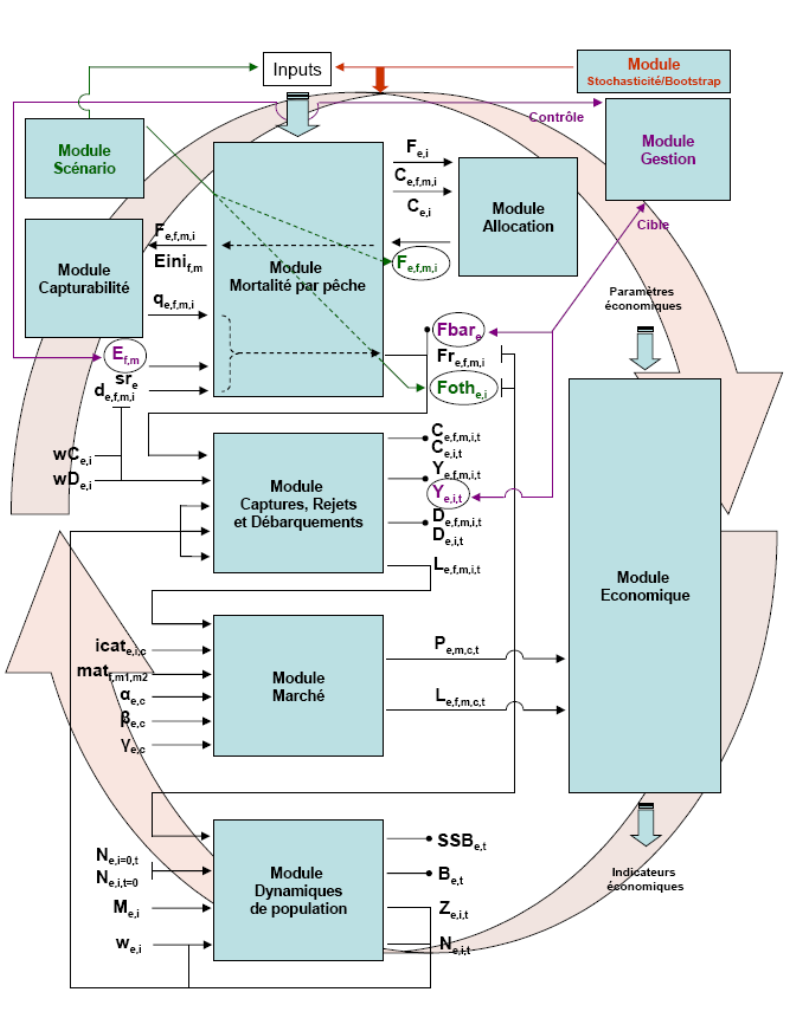
\includegraphics[width = 17cm]{figures/schema.png}
\end{center}
\caption{Schéma structurel simplifié du modèle bio-économique}
\label{fig:schema}
\end{figure}


\subsection{Module "Mortalité par pêche et Survie des rejets"}

Ce module fait appel à deux sous-modules. Le premier procède à la ventilation de la donnée "mortalité" initiale disponible par une variable auxiliaire supposée corrélée afin d’affiner le niveau de définition accessible. Ce processus s’effectue le plus souvent au moyen d’une variable de type "captures", ou à défaut, d’une donnée "débarquements". Le deuxième sous-module va estimer initialement une capturabilité associée afin de l’appliquer au cours du processus de modélisation à une variable de contrôle "effort". 

\subsubsection{Sous-module "Allocation de la mortalité"}

Avant tout, précisons que ce qui va se rapporter à cette étape d'allocation ne concerne que les dynamiques \textbf{XSA} et \textbf{SPiCT}. La mortalité par pêche pour la dynamique SS3 est d'entrée renseignée déjà ventilée au niveau flottille-métier-âge-cohorte-saison requis, aucun travail d'allocation n'est donc nécessaire. Le modèle statique quant à lui s'affranchit de cet indicateur puisqu'il se base sur des données de LPUE déjà disponibles au niveau flottille-métier. 

L’objectif de ce module est d’aboutir à un niveau de définition maximal du paramètre de mortalité, à savoir idéalement une valeur par espèce, âge, flottille et métier. Il existe plusieurs manières d’obtenir ce niveau maximal  (voir encadré \ref{bx:vent} décrivant les procédés de ventilation implémentés). En partant d’une donnée "Mortalité" plus précise, on peut se contenter d’une variable de ventilation plus grossière. On peut également procéder en deux étapes successives avec deux variables distinctes si la variable initiale ne décline que la dimension "âge", et qu'il reste donc à intégrer les dimensions "métier", puis "flottille". Toutes ces possibilités sont offertes par le module implémenté, et celui-ci considérera au mieux les ventilations à opérer le cas échéant.

Si nécessaire, une première ventilation sera effectuée au moyen des variables Cmi et Ci préalablement renseignées dans les onglets "Espèce" du fichier de paramétrage \todo{(voir partie 2)} afin d'intégrer au minimum la dimension "métier" à la donnée de mortalité par pêche. On rappelle qu'il s'agira idéalement de données de captures en nombre, mais qu'une autre donnée pourra à défaut être utilisée. Si à ce stade, la mortalité possède le niveau complet requis, la procédure s'arrêtera. Sinon, la seconde ventilation s’opérera avec les variables $Ymi$ et $Lref_{fe}$ (variable présente dans les onglets de paramétrage économique et appliquée ici à la matrice "fm" d'allocation flottille-métier) afin d'inclure la dimension "flottille". Il revient à l'utilisateur de s'assurer de la pertinence des données assignées à chacune de ces variables afin que le processus de ventilation aboutisse à des résultats justes et optimaux (cf encadré \ref{bx:vent} de la page suivante ).   

\textbf{\underline{Note :}} la ventilation ne s'effectue plus en tant qu'étape préliminaire aux simulations lors du lancement du modèle, mais désormais  lors de la phase d'intégration des indicateurs visant à créer l'objet R de paramétrage. Le paramètre calculé $F_{fmi}$ apparaît donc maintenant parmi les paramètres "sources" au sein de l'objet, et est au même titre qu'eux directement utilisé par le modèle.  

\begin{defbox}
    \textbf{\underline{Procédures de ventilation :}} ventilation d'une variable Mortalité (F) par une variable Capture (C)

	On décrit ici les procédures permettant de redéfinir le niveau d'agrégation d'une variable donnée en  prenant appui sur une donnée externe corrélée, de niveau de définition supérieur ou complémentaire. On prendra pour cela l'exemple d'une variable de mortalité par pêche, qu'on ventilera à l'aide d'une variable de captures totales. Ces méthodes d'application porteront sur différentes combinaisons de dimensions. Les dimensions illustrées seront d'indice "f" (flottille), "m" (métier) et "i" (âge).

    $\bullet$ Indice(s) en commun

    ~

    {\centering
        \begin{tabularx}{\textwidth}{|*{4}{>{\centering \arraybackslash}X|}}
        \hline
        \textbf{Variable à ventiler} & \textbf{Variable de ventilation} & \textbf{Variable complémentaire requise} & \textbf{Résultat} \\
        \textbf{($F$)} & \textbf{($C$)} & \textbf{($C_{tot}$)} & \textbf{($F_{ventil}$)}\\
         \hline
        $F_i$ & $C_{m,i}$ & $Ctot_i$ & $F_{m,i}$ \\ \hline
        $F_i$ & $C_{f,m,i}$ & $Ctot_i$ & $F_{f,m,i}$ \\ \hline
        $F_{m,i}$ & $C_{f,m}$ & $Ctot_m$ & $F_{f,m,i}$ \\ \hline
        $F_{m,i}$ & $C_{f,m,i}$ & $Ctot_{m,i}$ & $F_{f,m,i}$ \\
        \hline
        \end{tabularx}
    }

    $\bullet$ Pas d'indices en commun

    ~

    {\centering
    \begin{tabularx}{\textwidth}{|*{4}{>{\centering \arraybackslash}X|}}
        \hline
        $F_i$ & $C_m$ & $Ctot$ & $F_{m,i}$ \\ \hline
        $F_i$ & $C_{f,m}$ & $Ctot$ & $F_{f,m,i}$ \\ \hline
        $F_{m,i}$ & $C_f$ & $Ctot$ & $F_{f,m,i}$ \\
        \hline
        \end{tabularx}
    }

    \textbf{\underline{Equation :}}

    $$
        F_{ventil} = \frac{ F \times C}{Capt_{tot}} \text{ sur tous les indices en présence}
    $$
    \label{bx:vent}

    ~

    {\centering \textbf{Méthodologie appliquée dans la procédure de ventilation}}
\end{defbox}


$\bullet$ \textbf{Paramètres initiaux} (la description des paramètres d'entrée et l'équation de calcul associée dépeignant ici la procédure d'allocation ne doivent être considérées que comme un cas particulier d'une ventilation en une étape)

$\bullet$ \textbf{XSA, SPiCT}

\begin{iTable}{0.17}{0.5}{0.33}
    \text{\normalsize\textbf{Notation}} & \textbf{Description} & \textbf{Source} \tabnl

    F_{e,i} & Coefficient de mortalité par pêche initial (ici, par espèce et par âge) 
    & Stock Assessment ($i = \{all\}$ pour modèle global SpiCT, et $\{i\} = \{0,1,...\}$ pour modèle aux âges XSA) \tabnl
    C_{e,f,m,i} & Variable de ventilation à un niveau de définition requis (ici, captures par espèce, flottille, métier et âge) & SACROIS \tabnl
    Ctot_{e,i} & Variable de ventilation totale (doit être définie sur l’intersection des niveaux des deux variables précédentes) & SACROIS \tabnl
  
    \caption{Paramètres initiaux XSA, SPiCT pour le sous-module "allocation de la mortalité par pêche"}
\end{iTable}

$\bullet$ \textbf{SS3} (toutes les variables décrites ci-dessous comprennent chacune 4x4 incarnations correspondants aux combinaisons "cohorte  / saison" ; par souci d'identification, les noms de ces variables seront indexées M1S1, M1S2, …, M4S3, M4S4):

\begin{iTable}{0.17}{0.5}{0.33}
    \text{\normalsize\textbf{Notation}} & \textbf{Description} & \textbf{Source} \tabnl

    iniFq_{e,i} & Coefficient de mortalité par pêche total initial (par espèce, âge, saison et cohorte) & Stock Assessment \tabnl
    Fq_{e,i} & Coefficient de mortalité par pêche total à $t=1$ (par espèce, âge, saison et cohorte) & Stock Assessment \tabnl
    iniFq_{e,i} & Coefficient de mortalité par pêche total initial (par espèce, flottille, métier, âge, saison et cohorte) & Stock Assessment \tabnl
    Fq_{e,f,m,i} & Coefficient de mortalité par pêche total à $t=1$ (par espèce, flottille, métier, âge, saison et cohorte) & Stock Assessment \tabnl

    iniFqLwt_{e,i} & Coefficient de mortalité par pêche "poids débarqués" initial (par espèce, âge, saison et cohorte) & Stock Assessment \tabnl
    FqLwt_{e,i} & Coefficient de mortalité par pêche "poids débarqués" à $t=1$ (par espèce, âge, saison et cohorte) & Stock Assessment \tabnl
    iniFqLwt_{e,f,m,i} & Coefficient de mortalité par pêche "poids débarqués" initial (par espèce, flottille, métier, âge, saison et cohorte) & Stock Assessment \tabnl
    FqLwt_{e,f,m,i} & Coefficient de mortalité par pêche "poids débarqués" à $t=1$ (par espèce, flottille, métier, âge, saison et cohorte) & Stock Assessment \tabnl

    iniFqDwt_{e,i} & Coefficient de mortalité par pêche "poids rejetés" initial (par espèce, âge, saison et cohorte) & Stock Assessment \tabnl
    FqDwt_{e,i} & Coefficient de mortalité par pêche "poids rejetés" à $t=1$ (par espèce, âge, saison et cohorte) & Stock Assessment \tabnl
    iniFqDwt_{e,f,m,i} & Coefficient de mortalité par pêche "poids rejetés" initial (par espèce, flottille, métier, âge, saison et cohorte) & Stock Assessment \tabnl
    FqDwt_{e,f,m,i} & Coefficient de mortalité par pêche "poids rejetés" à $t=1$ (par espèce, flottille, métier, âge, saison et cohorte) & Stock Assessment \tabnl
  
    \caption{Paramètres initiaux SS3 pour le sous-module "allocation de la mortalité par pêche"}
\end{iTable}

\hspace{10mm}$\bullet$ \textbf{Variables calculées (XSA et SPiCT)} 

\begin{cTable}{0.17}{0.09}{0.33}{0.4}
    \text{\normalsize\textbf{Notation}} & \textbf{Type} & \textbf{Description} & \text{\normalsize\textbf{Equation}} \tabnl

    F_{e,f,m,i} & Sortie & Coefficient instantané de mortalité par pêche ventilé initial (ici, par espèce, flottille, métier et âge) & 
    F_{e,f,m,i} = \frac{F_{e,i} \cdot C_{e,f,m,i}}{Ctot_{e,i}} \tabnl
    Foth_{e,i} & Sortie & Mortalité par pêche initiale "autres flottilles" par espèce et âge. Entrée des modules \textit{Captures} et \textit{Dynamiques de populations} & 
    Foth_{e,i} = F_{e,i} - \sum_{f,m} F_{e,f,m,i} \tabnl

    \caption{Paramètres calculés pour le sous-module "allocation de la mortalité par pêche"}
\end{cTable}


\subsubsection{Sous-module "Calcul de capturabilité"}

On utilise ici le terme "capturabilité" de façon générique pour désigner la mortalité par pêche ramenée à une unité d'effort donnée. Cet effort sera le produit de deux variables d'entrée effort1 et effort2, auxquelles on pourra affecter différents couples d'indicateurs (voir tableau \ref{tab:icaptu} ci-dessous). La mortalité par pêche devient ainsi une fonction de la variable d’effort au cours du processus implémenté.

\hspace{10mm}$\bullet$ \textbf{Paramètres initiaux (XSA, SPiCT,SS3)} 

\begin{iTable}{0.17}{0.5}{0.33}
    \text{\normalsize\textbf{Notation}} & \textbf{Description} & \textbf{Source} \tabnl

    effort1_{f,m} & Première composante d'effort (ici au niveau flottille-métier), soit le nombre de marées moyen par an et par navire ($nbTrip$) soit le nombre de jours de mer moyen par an et par navire ($nbds$). & SACROIS \tabnl
    effort2_{f,m} & Deuxième composante d'effort (ici au niveau flottille-métier), soit la durée moyenne des marées par an et par navire ($tripLgth$) soit l'élément neutre 1 & SACROIS \tabnl

    \caption{Paramètres initiaux SS3 pour le sous-module "calcul de capturabilité"}
    \label{tab:icaptu}
\end{iTable}

\hspace{10mm}$\bullet$ \textbf{Variables calculées (XSA et SPiCT, SS3 sur les variables mortalités)} 

\begin{cTable}{0.17}{0.09}{0.33}{0.4}
    \text{\normalsize\textbf{Notation}} & \textbf{Type} & \textbf{Description} & \text{\normalsize\textbf{Equation}} \tabnl

    Q_{e,f,m,i} & Sortie & Capturabilité initiale (par espèce, flottille, métier et âge) & 
    Q_{e,f,m,i} = \frac{F_{e,f,mi}  }{ effort1_{f,m} \times effort2_{f,m} } \tabnl

    \caption{Paramètres calculés pour le sous-module "calcul de capturabilité"}
\end{cTable}

\subsubsection{Module "Mortalité par pêche"} \label{sec:mortalsub}

Ce module intègre la méthode de calcul des capturabilités décrite précédemment. Il va en outre évaluer les mortalités par pêche corrigées. Le paramétrage systématisant dorénavant pour une flottille donnée la description exhaustive des espèces pêchées et des métiers pratiqués (via une espèce "ZZZ" considérée et un métier "Autres"), la couverture des indicateurs de sortie du modèle définis par flottille est complète.  Ainsi, les mortalités complémentaires, au même titre que les autres variables complémentaires que le modèle sera amené à évaluer, sont désormais uniquement celles engendrées par les flottilles non modélisées. à partir de la mortalité par pêche ventilée initialement. Le module procède également au calcul de l'indicateur "Fbar" pour chacune des espèces modélisées XSA ou SS3.
	
Ajoutons que les deux variables de sortie "Mortalité par pêche  ventilée» (F) et "Mortalité par pêche Autres flottilles" (Foth) sont des paramètres internes (donc non renseignés dans le fichier de paramétrage car évalués lors de la construction de l'objet input) sur lesquels il est possible d'intervenir au moyen du module "Scénario". On décrira le mode opératoire de ce module dans le chapitre correspondant. Il faut simplement noter que de cette manière,  l'utilisateur pourra par exemple intégrer dans la simulation la prise en compte d'un facteur de sélectivité à un niveau flottille-métier-âge pour une ou plusieurs espèces modélisées.  

$\bullet$ \textbf{XSA}
\hspace{10mm}$\bullet$ \textbf{Paramètres initiaux (inputs biologiques prélevés dans les feuillets de paramétrage Stocks)} 

\begin{iTable}{0.17}{0.5}{0.33}
    \text{\normalsize\textbf{Notation}} & \textbf{Description} & \textbf{Source} \tabnl

    d_{e,f,m,i} & Pourcentage de captures totales rejetées en nombre (par espèce, flottille, métier et âge) & Stock Assessment \tabnl
    doth_i & Pourcentage de captures totales rejetées en nombre (par âge sur l'ensemble des flottilles non modélisés) & Stock Assessment \tabnl
    sr_e & Taux de survie des rejets (par espèce) & Stock Assessment \tabnl
    E_{f,m} & Effort (par flottille et métier, produit d'$effort1$ et d'$effort2$) & SACROIS \tabnl
    p_{e,i} & Pondération pour le calcul du Fbar par espèce (ie 1 pour les âges à considérer, 0 pour les autres) & Stock Assessment \tabnl

    \caption{Paramètres initiaux XSA pour le module "Mortalité par pêche"}
\end{iTable}

\hspace{10mm}$\bullet$ \textbf{Variables calculées} 

\begin{cTable}{0.17}{0.09}{0.33}{0.4}
    \text{\normalsize\textbf{Notation}} & \textbf{Type} & \textbf{Description} & \text{\normalsize\textbf{Equation}} \tabnl

    F_{e,f,m,i,t} & Sortie & Mortalité par pêche (par espèce, flottille, métier et âge, à l’instant $t$). Entrée des modules \textit{Captures} et \textit{Dynamiques de populations} & 
    F_{e,f,m,i,t} =  q_{e,f,m,i} \cdot E_{f,m,t} \tabnl
    K_{e,f,m,i} & Interne & Facteur de correction de la mortalité par pêche lié à la survie des rejets. & 
    K_{e,f,m,i} = 1 - sr_e \cdot d_{e,f,m,i} \tabnl
    Fr_{e,f,m,i,t} & Sortie & Mortalité par pêche corrigée (par espèce, flottille, métier et âge, à l’instant $t$). Entrée des modules \textit{Captures} et \textit{Dynamiques de populations} & 
    Fr_{e,f,m,i,t} = F_{e,f,m,i,t} \cdot K_{e,f,m,i} \tabnl
    Froth_{e,i} & Sortie & Mortalité par pêche initiale "autres flottilles" corrigée par espèce et âge. Entrée des modules \textit{Captures} et \textit{Dynamiques de populations} & 
    Froth_{e,i} = Froth_{e,i} \cdot(1- sr_e \cdot doth_i) \tabnl
    Fbar_{e,t} & Sortie & Taux de mortalité par pêche par espèce. & 
    Fbar_{e,t} = \frac{1}{\sum_i p_{e,i}} \sum_i p_{e,i} \cdot (\sum_{f,m} Fr_{e,f,m,i} + Froth_{e,i} ) \tabnl

    \caption{iParamètres calculés XSA pour le module "Mortalité par pêche"}
\end{cTable}


$\bullet$ \textbf{SPiCT}

\hspace{10mm}$\bullet$ \textbf{Paramètres initiaux (inputs biologiques prélevés dans les feuillets de paramétrage Stocks)} 

\begin{iTable}{0.17}{0.5}{0.33}
    \text{\normalsize\textbf{Notation}} & \textbf{Description} & \textbf{Source} \tabnl

    d_{e} & Pourcentage de captures totales rejetées sur les flottilles modélisées (par espèce) & Stock Assessment \tabnl
    doth_e & Pourcentage de captures totales rejetées sur l'ensemble des flottilles non modélisés (par espèce) & Stock Assessment \tabnl

    \caption{Paramètres initiaux SPiCT pour le module "Mortalité par pêche"}
\end{iTable}

\hspace{10mm}$\bullet$ \textbf{Variables calculées} 

\begin{cTable}{0.17}{0.09}{0.33}{0.4}
    \text{\normalsize\textbf{Notation}} & \textbf{Type} & \textbf{Description} & \text{\normalsize\textbf{Equation}} \tabnl

    F_{e,f,m,i,t} & Sortie & Mortalité par pêche (par espèce, flottille, métier et âge, à l’instant $t$). Entrée des modules \textit{Captures} et \textit{Dynamiques de populations} & 
    F_{e,f,m,i,t} = q_{e,f,m,i,t} \times F_{f,m,t}  \tabnl
    Foth_{e,i} & Sortie & Mortalité par pêche initiale "autres flottilles" par espèce et âge. Entrée des modules \textit{Captures} et \textit{Dynamiques de populations} & 
    Foth_{e,i} = F_{e,i} - \sum_{f,m} F_{e,f,m,i,0}  \tabnl

    \caption{Paramètres calculés SPiCT pour le module "Mortalité par pêche"}
\end{cTable}

$\bullet$ \textbf{SS3}

\hspace{10mm}$\bullet$ \textbf{Paramètres initiaux (inputs biologiques prélevés dans les feuillets de paramétrage Stocks)} 

\underline{Note :} les paramètres biologiques SS3 se définissent sur des dimensions supplémentaires "saison" (indice 's', 4 modalités) et "cohorte" (indice 'mo' pour 'morph', 4 modalités)

\begin{iTable}{0.17}{0.5}{0.33}
    \text{\normalsize\textbf{Notation}} & \textbf{Description} & \textbf{Source} \tabnl

    iniFq_{e,i,s,mo} & Mortalité par pêche initiale "captures en nombre" (par espèce, âge, saison et cohorte) & Stock Assessment \tabnl
    Fq_{e,i,s,mo} & Mortalité par pêche projection ($t>0$) "captures en nombre" (par espèce, âge, saison et cohorte) & Stock Assessment \tabnl
    iniFq\newline_{e,f,m,i,s,mo} & Mortalité par pêche initiale "captures en nombre" (par espèce, flottille, métier, âge, saison et cohorte) & Stock Assessment \tabnl
    Fq_{e,f,m,i,s,mo} & Mortalité par pêche projection ($t>0$) "captures en nombre" (par espèce, flottille, métier, âge, saison et cohorte) & Stock Assessment \tabnl
    iniFqLwt\newline_{e,i,s,mo} & Mortalité par pêche initiale "poids débarqués" (par espèce, âge, saison et cohorte) & Stock Assessment \tabnl
    FqLwt\newline_{e,i,s,mo} & Mortalité par pêche projection ($t>0$) "poids débarqués" (par espèce, âge, saison et cohorte) & Stock Assessment \tabnl
    iniFqLwt\newline_{e,f,m,i,s,mo} & Mortalité par pêche initiale "poids débarqués" (par espèce, flottille, métier, âge, saison et cohorte) & Stock Assessment \tabnl
    FqLwt\newline_{e,f,m,i,s,mo} & Mortalité par pêche projection ($t>0$) "poids débarqués" (par espèce, flottille, métier, âge, saison et cohorte) & Stock Assessment \tabnl
    iniFqDwt\newline_{e,i,s,mo} & Mortalité par pêche initiale "poids rejetés" (par espèce, âge, saison et cohorte) & Stock Assessment \tabnl
    FqDwt_{e,i,s,mo} & Mortalité par pêche projection ($t>0$) "poids rejetés" (par espèce, âge, saison et cohorte) & Stock Assessment \tabnl
    iniFqDwt\newline_{e,f,m,i,s,mo} & Mortalité par pêche initiale "poids rejetés" (par espèce, flottille, métier, âge, saison et cohorte) & Stock Assessment \tabnl
    FqDwt\newline_{e,f,m,i,s,mo} & Mortalité par pêche projection ($t>0$) "poids rejetés" (par espèce, flottille, métier, âge, saison et cohorte) & Stock Assessment \tabnl

    \caption{Paramètres initiaux SS3 pour le module "Mortalité par pêche"}
\end{iTable}

\hspace{10mm}$\bullet$ \textbf{Variables calculées} 

\begin{cTable}{0.17}{0.09}{0.33}{0.4}
    \text{\normalsize\textbf{Notation}} & \textbf{Type} & \textbf{Description} & \text{\normalsize\textbf{Equation}} \tabnl

    iniFothq\newline_{e,i,s,mo} & - & Mortalité par pêche initiale "captures en nombre – Autres flottilles" (par espèce, âge, saison et cohorte) & 
    iniFothq_{e,i,s,mo} = iniFq_{e,i,s,mo}  - \sum_{f,m} iniFq_{e,f,m,i,s,mo} \tabnl
    Fothq\newline_{e,i,s,mo} & - & Mortalité par pêche projection ($t>0$) "captures en nombre – Autres flottilles" (par espèce, âge, saison et cohorte) & 
    Fothq_{e,i,s,mo} = Fq_{e,i,s,mo}  - \sum_{f,m} Fq_{e,f,m,i,s,mo}  \tabnl
    iniFothqLwt\newline_{e,i,s,mo} & - & Mortalité par pêche initiale "poids débarqués – Autres flottilles" (par espèce, âge, saison et cohorte) & 
    iniFothqLwt_{e,i,s,mo} = iniFqLwt_{e,i,s,mo} - \sum_{f,m} iniFqLwt_{e,f,m,i,s,mo} \tabnl
    FothqLwt\newline_{e,i,s,mo} & - & Mortalité par pêche projection ($t>0$) "poids débarqués – Autres flottilles" (par espèce, âge, saison et cohorte) & 
    FothqLwt_{e,i,s,mo} = FqLwt_{e,i,s,mo} - \sum_{f,m} FqLwt_{e,f,m,i,s,mo} \tabnl
    iniFothqDwt\newline_{e,i,s,mo} & - & Mortalité par pêche initiale "poids rejetés – Autres flottilles" (par espèce, âge, saison et cohorte) & 
    iniFothqDwt_{e,i,s,mo} = iniFqDwt_{e,i,s,mo} - \sum_{f,m} iniFqDwt_{e,f,m,i,s,mo} \tabnl
    FothqDwt\newline_{e,i,s,mo} & - & Mortalité par pêche projection ($t>0$) "poids rejetés – Autres flottilles" (par espèce, âge, saison et cohorte) & 
    FothqDwt_{e,i,s,mo} = FqDwt_{e,i,s,mo} - \sum_{f,m} FqDwt_{e,f,m,i,s,mo} \tabnl

    \caption{Paramètres calculés SS3 pour le module "Mortalité par pêche"}
\end{cTable}

Précisons enfin que les espèces dites "statiques" ne s'inscrivent pas dans ce module.

\subsection{Module "Dynamique de populations"}

\subsubsection{Module principal}

Ce module  se charge d'opérer le calcul des indicateurs relatifs aux stocks des espèces considérées dynamiquement dans la simulation (XSA et SS3). En partant de la mortalité par pêche appliquée au stock et estimée en sortie du module décrit dans le chapitre précédent , il estime pour chaque pas de temps, et à partir d'un état initial, la mortalité totale, les effectifs totaux aux âges, la biomasse et la biomasse reproductrice résultantes. Notons qu'il est possible de définir dans le fichier de paramétrage un recrutement a priori par espèce pour les projections (cf première ligne du tableau \ref{tbl:xsadyna}).  Toutefois, si le module "Recrutement" est activé (voir \ref{sec:recrut}), le module principal fera appel à lui au cours de la simulation afin d'estimer $N_{e,i=0,t}$ pour tout instant non initial (fonctionnel uniquement pour la dynamique XSA) 

$\bullet$ \textbf{XSA} 

\hspace{10mm}$\bullet$ \textbf{Paramètres initiaux} 

\begin{iTable}{0.17}{0.5}{0.33}
    \text{\normalsize\textbf{Notation}} & \textbf{Description} & \textbf{Source} \tabnl

    N_{e,i,t=0} \newline\text{ et } N_{e,i=0,t} & Effectifs initiaux en nombre par espèce et par âge, et  effectifs des recrutements par espèce à l'instant $t$. & Stock Assessment \tabnl
    M_{e,i} & Taux de mortalité naturelle par espèce et par âge & Stock Assessment \tabnl
    w_{e,i} & Poids moyen dans le stock par espèce à l’âge $i$ & Stock Assessment \tabnl
    mr_{e,i} & Taux de maturité dans le stock par espèce à l’âge $i$ & Stock Assessment \tabnl

    \caption{Paramètres initiaux XSA pour le module "Dynamique de populations"}
    \label{tbl:xsadyna}
\end{iTable}

\hspace{10mm}$\bullet$ \textbf{Variables calculées} 

\begin{cTable}{0.17}{0.09}{0.33}{0.4}
    \text{\normalsize\textbf{Notation}} & \textbf{Type} & \textbf{Description} & \text{\normalsize\textbf{Equation}} \tabnl

    Z_{e,i,t} & Sortie & Coefficient de mortalité totale (par espèce et âge à l’instant t). Entrée du module Captures. 
    & Z_{e,i,t} = M_{e,i} + \sum_{f,m} Fr_{ef,f,i,t}  + Froth_{e,i,t}\tabnl
    N_{e,i,t} & Sortie & Effectif en nombre du groupe d’âge i à l’instant t par espèce. 
    & N_{e,i+1,t=1} = N_{e,i,t} \cdot e^{-Z_{e,i,t}} \newline 
    \text{---------------------------------------------} \newline
    N_{e,i+1,t+1} = N_{e,i,t} \cdot e^{-Z_{e,i,t}} + N_{e,i+1,t} \cdot e^{-Z_{e,i+1,t}} \newline \text{pour le groupe d'âge +}  \tabnl
    B_{e,t} & Sortie & Biomasse à l’instant t par espèce. 
    & B_{e,t} = \sum_i N_{e,i,t} \cdot w_{e,i} \tabnl
    SSB_{e,t} & Sortie & Biomasse reproductrice à l’instant t par espèce. 
    & SSB_{e,t}= \sum_i N_{e,i,t} \cdot w_{e,i} \cdot mr_{e,i} \tabnl

    \caption{Paramètres calculés XSA pour le module "Dynamique de populations"}
\end{cTable}


$\bullet$ \textbf{SPiCT} 

\hspace{10mm}$\bullet$ \textbf{Paramètres initiaux} 

\begin{iTable}{0.17}{0.5}{0.33}
    \text{\normalsize\textbf{Notation}} & \textbf{Description} & \textbf{Source} \tabnl

    B_{e,t=0} & Biomasse à l’instant initial par espèce. & Stock Assessment \tabnl
    r_e & Taux de croissance intrinsèque par espèce. & Stock Assessment \tabnl
    K_e & Capacité de charge par espèce. & Stock Assessment \tabnl
    n_e & Paramètre de détermination de la forme de la courbe de production, par espèce. & Stock Assessment \tabnl

    \caption{Paramètres initiaux SPiCT pour le module "Dynamique de populations"}
\end{iTable}

\hspace{10mm}$\bullet$ \textbf{Variables calculées} 

\begin{cTable}{0.17}{0.09}{0.33}{0.4}
    \text{\normalsize\textbf{Notation}} & \textbf{Type} & \textbf{Description} & \text{\normalsize\textbf{Equation}} \tabnl

    B_{e,t} & Sortie & Biomasse à l’instant t par espèce. & 
    B_{e,t} = B_{e,t-1} \times ( 1 + \frac{r_e}{n_e -1} \cdot (1 - [\frac{B_{e,t-1}}{K_e}] ^{ n_e - 1}) - F_{e,t-1} \tabnl

    \caption{Paramètres calculés SPiCT pour le module "Dynamique de populations"}
\end{cTable}

$\bullet$ \textbf{SS3} 

\hspace{10mm}$\bullet$ \textbf{Paramètres initiaux} 

\begin{iTable}{0.17}{0.5}{0.33}
    \text{\normalsize\textbf{Notation}} & \textbf{Description} & \textbf{Source} \tabnl

    IniN_{e,i,s,mo,t=0} & Effectifs initiaux en nombre par espèce et par âge, saison et cohorte. & Stock Assessment \tabnl
    N_{e,i,s=1,mo,t=1} & Effectifs de projection initiaux ($t>0$, saison 1) en nombre par espèce, par âge et cohorte. & Stock Assessment \tabnl
    N_{e,i=0,s,mo=s} & Recrutement par saison en nombre. & Stock Assessment \tabnl
    matWt_{e,i,mo} & Poids moyen pondéré pour calcul de la SSB par espèce, âge et cohorte. & Stock Assessment \tabnl
    M_{e,i,mo} & Taux de mortalité naturelle par espèce, par âge et cohorte. & Stock Assessment \tabnl

    \caption{Paramètres initiaux SS3 pour le module "Dynamique de populations"}
\end{iTable}

\hspace{10mm}$\bullet$ \textbf{Variables calculées} (pour $t>0$ . A $t=0$, les versions "ini" des variables de mortalité sont utilisées)

\begin{cTable}{0.17}{0.09}{0.33}{0.4}
    \text{\normalsize\textbf{Notation}} & \textbf{Type} & \textbf{Description} & \text{\normalsize\textbf{Equation}} \tabnl

    Z_{e,i,s,mo,t} & Sortie & Coefficient de mortalité totale (par espèce et âge, saison, cohorte à l’instant t). Entrée du module \textit{Captures}. & 
    Z_{e,i,s,mo,t} = M_{e,i,mo} + \sum_{f,m}  Fq_{e,f,m,i,s,mo,t} + Fq_{e,i,s,mo,t} \tabnl
    auxiA_{e,i,s,mo,t} & Interne & Variable de calcul intermédiaire. & 
    auxiA_{e,i,s,mo,t} = N_{e,i,s,mo,t} \times exp^{- Z_{e,i,s,mo,t} / 4} \tabnl
    N_{e,i,s,mo,t} & Sortie & Effectif en nombre par espèce et âge, saison, cohorte à l’instant $t$. & 
    N_{e,i,s+1,mo,t} = auxiA_{e,i,s,mo,t} + N_{e,i,s+1,mo,t} \cdot 1_{i=0 \cap mo =s+1}\newline \text{ si } s<4 \newline
    \text{---------------------------------------------} \newline
    N_{e,i,s=1,mo,t+1} = auxiA_{e,i-1,s=4,mo,t} + auxiA_{e,i,s=4,mo,t} \cdot 1_{i='gp+'} \newline \text{ sinon } \tabnl
    SSB_{e,t} & Sortie & Biomasse reproductrice à l’instant $t$ par espèce. & 
    SSB_{e,t} = \sum_{i,mo}  matWt_{e,i,mo} \times N_{e,i,s=1,mo,t} \tabnl
    Fss3_{e,f,m,i} & Sortie & Mortalité par pêche annuelle aux âges "captures en nombre" (par espèce, flottille, métier, âge) & 
    Fss3_{e,f,m,i} = \sum_s \frac{ \sum_{mo}  Fq_{e,f,m,i,s,mo} \times N_{e,i,s,mo} }{ 4 \times \sum_{mo}  N_{e,i,s,mo} } \tabnl
    Fothss3_{e,i} & Sortie & Mortalité par pêche annuelle aux âges "captures en nombre - Autres flottilles" (par espèce et âge) & 
    Fothss3_{e,i} = \sum_s \frac{ \sum_{mo}  Fq_{e,i,s,mo} }{ 4 \times \sum_{mo}  N_{e,i,s,mo} } \tabnl
    Fbar_{e,t} & Sortie & Taux de mortalité par pêche par espèce et âge. & 
    Fbar_{e,t} = \frac{1}{\sum_i p_{e,i}} \sum_i p_{e,i} \cdot (\sum_{f,m} Fss3_{e,f,m,i} + Fothss3_{e,i} ) \tabnl

    \caption{Paramètres calculés SS3 pour le module "Dynamique de populations"}
\end{cTable}


\subsubsection{Module "Recrutement} \label{sec:recrut}

Le module "Recrutement" est une composante du module composite "Stochasticité/Bootstrap" qui va donner la possibilité à l'utilisateur de générer un recrutement pour une espèce donnée, de manière stochastique, et ce à tout instant non initial, qui sera intégré en tant qu'input du modèle (voir illustration sur le schéma \ref{fig:schema}). Ce module propose pour l'instant deux méthodes de génération de recrutement dit "aléatoire". L'utilisateur peut ainsi assigner à chacune des espèces modélisées un type de recrutement donné avec des paramètres qui lui sont propres.
	
La première méthode va gérer les recrutements issus de relations stock-recrutement. Elle permet, pour le moment, de choisir entre 5 types de relations paramétrables (recrutement moyen, de type Hockey Stick, Beverton \& Holt, Ricker, et Shepherd), et autorise l'adjonction d'un bruit paramétrable.
	
La seconde option permet de procéder aux générations par tirage aléatoire. Il est alors possible de réaliser un tirage aléatoire dans un historique de recrutement renseigné dans le fichier de paramétrage (le tirage aléatoire pouvant s'effectuer indépendamment ou non par espèce), ou encore d'envisager le recrutement comme la réalisation d'une variable aléatoire de loi et de paramètre(s) choisis par l'utilisateur.
	
Précisons enfin que ce module "Recrutement" n'est pour le moment applicable que sur les dynamiques de type XSA.


\subsection{Module "Captures, débarquements et rejets"}

A l'inverse du module précédent qui s'appliquait essentiellement du point de vue du stock, le module ici abordé se place du point de vue de l'engin de pêche. Des indicateurs de captures (en nombre et en poids) calculés sont déduites les quantités retenues et les quantités rejetées. En outre, les données de captures sont disponibles pour deux niveaux d'agrégation, l'une intégrant ainsi les captures des flottilles et métiers non modélisés.

$\bullet$ \textbf{XSA}

\hspace{10mm}$\bullet$ \textbf{Paramètres initiaux} 

\begin{iTable}{0.17}{0.5}{0.33}
    \text{\normalsize\textbf{Notation}} & \textbf{Description} & \textbf{Source} \tabnl

    wD_{e,i} & Poids moyen des individus dans la fraction rejetée par espèce à l’âge $i$ & Stock Assessment \tabnl
    wC_{e,i} & Poids moyen des individus dans la capture par espèce à l’âge $i$ & Stock Assessment \tabnl


    \caption{Paramètres initiaux XSA pour le module "Captures, débarquements et rejets"}
\end{iTable}

\hspace{10mm}$\bullet$ \textbf{Variables calculées} 

\begin{cTable}{0.17}{0.09}{0.33}{0.4}
    \text{\normalsize\textbf{Notation}} & \textbf{Type} & \textbf{Description} & \text{\normalsize\textbf{Equation}} \tabnl

    C_{e,f,m,i,t} & Sortie & Captures en nombre (par espèce, flottille, métier et âge, sur la période $t$). & 
    C_{e,f,m,i,t} = \frac{F_{e,f,m,i,t}}{Z_{e,i,t}} \times N_{e,i,t} \times (1-e^{-Z_{e,i,t}}) \tabnl
    C_{e,i,t} & Sortie & Captures en nombre (par espèce et âge, sur la période $t$). & 
    C_{e,i,t} = \frac{ \sum_{f,m} F_{e,f,m,i,t} + Foth_{e,i} }{Z_{e,i,t}} \times N_{e,i,t} \times (1-e^{-Z_{e,i,t}}) \tabnl
    Y_{e,f,m,i,t} & Sortie & Captures en poids (par espèce, flottille, métier et âge, sur la période $t$). & 
    Y_{e,f,m,i,t} = wC_{e,i} \times C_{e,f,m,i,t} \tabnl
    Y_{e,i,t} & Sortie & Captures en poids (par espèce et âge sur la période $t$). & 
    Y_{e,i,t} = wC_{e,i} \times C_{e,i,t} \tabnl
    D_{e,f,m,i,t} & Sortie & Rejets en poids (par espèce, flottille, métier et âge, sur la période $t$). & 
    D_{e,f,m,i,t} = d_{e,f,m,i} \times wD_{e,i} \times C_{e,f,m,i,t} \newline \text{si } wD_{e,i} \text{ disponible} \newline
    \text{---------------------------------------------} \newline
    D_{e,f,m,i,t} = d_{e,f,m} \times Y_{e,f,m,t} \text{ sinon} \tabnl
    L_{e,f,m,i,t} & Sortie & Débarquements en poids (par espèce, flottille, métier et âge, sur la période $t$). Entrée du module \textit{Marché}. & 
    L_{e,f,m,i,t} = Y_{e,f,m,i,t} - D_{e,f,m,i,t} \tabnl

    \caption{Paramètres calculés XSA pour le module "Captures, débarquements et rejets"}
\end{cTable}

$\bullet$ \textbf{SPiCT}

\hspace{10mm}$\bullet$ \textbf{Paramètres initiaux} 

\begin{iTable}{0.17}{0.5}{0.33}
    \text{\normalsize\textbf{Notation}} & \textbf{Description} & \textbf{Source} \tabnl

    d_{e,f,m} & Pourcentage de captures totales rejetées en poids (par espèce, flottille, métier) & Stock Assessment \tabnl

    \caption{Paramètres initiaux SPiCT pour le module "Captures, débarquements et rejets"}
\end{iTable}

\hspace{10mm}$\bullet$ \textbf{Variables calculées} 

\begin{cTable}{0.17}{0.09}{0.33}{0.4}
    \text{\normalsize\textbf{Notation}} & \textbf{Type} & \textbf{Description} & \text{\normalsize\textbf{Equation}} \tabnl

    Y_{e,f,m,t} & Sortie & Captures en poids (par espèce, flottille, métier sur la période $t$). & 
    Y_{e,f,m,t} = F_{e,f,m,t} \times B_{e,t} \tabnl
    Y_{e,t} & Sortie & Captures en poids (par espèce sur la période $t$). & 
    Y_{e,t} = (\sum_{f,m} F_{e,f,m,t} + Froth_{e,t} ) \times B_{e,t} \tabnl
    D_{e,f,m,t} & Sortie & Rejets en poids (par espèce, flottille, métier et âge, sur la période $t$). & 
    D_{e,f,m,t} = d_{e,f,m} \times Y_{e,f,m,t} \tabnl
    L_{e,f,m,t} & Sortie & Débarquements en poids (par espèce, flottille, métier et âge, sur la période $t$). Entrée du module \textit{Marché}. & 
    L_{e,f,m,t} = Y_{e,f,m,t} - D_{e,f,m,t} \tabnl

    \caption{Paramètres calculés SPiCT pour le module "Captures, débarquements et rejets"}
\end{cTable}

$\bullet$ \textbf{SS3}

\begin{cTable}{0.17}{0.09}{0.33}{0.4}
    \text{\normalsize\textbf{Notation}} & \textbf{Type} & \textbf{Description} & \text{\normalsize\textbf{Equation}} \tabnl

    C_{e,f,m,i,t} & Sortie & Captures en nombre (par espèce, flottille, métier et âge, sur la période $t$). & 
    C_{e,f,m,i,t} = \sum_{s,mo} ( \frac{Fq_{e,f,m,i,s,mo,t}}{Z_{e,i,s,mo,t}} \times N_{e,i,s,mo,t} \times (1-e^{-Z_{e,i,s,mo,t} / 4}) ) \tabnl
    C_{e,i,t} & Sortie & Captures en nombre (par espèce et âge, sur la période $t$). & 
    C_{e,i,t} = \sum_{s,mo} ( \frac{ Fq_{e,f,m,i,s,mo,t} -M_{e,i,mo} }{Z_{e,i,s,mo,t}} \times N_{e,i,s,mo,t} \times (1-e^{-Z_{e,i,s,mo,t} / 4}) ) \tabnl

    L_{e,f,m,i,t} & Sortie & Débarquements en poids (par espèce, flottille, métier et âge, sur la période $t$). Entrée du module \textit{Marché}. & 
    L_{e,f,m,i,t} = \sum_{s,mo} ( \frac{FqLwt_{e,f,m,i,s,mo,t}}{Z_{e,i,s,mo,t}} \times N_{e,i,s,mo,t} \times (1-e^{-Z_{e,i,s,mo,t} / 4}) ) \tabnl
    D_{e,f,m,i,t} & Sortie & Rejets en poids (par espèce, flottille, métier et âge, sur la période $t$). & 
    D_{e,f,m,i,t} = \sum_{s,mo} ( \frac{FqDwt_{e,f,m,i,s,mo,t}}{Z_{e,i,s,mo,t}} \times N_{e,i,s,mo,t} \times (1-e^{-Z_{e,i,s,mo,t} / 4}) ) \tabnl
    Y_{e,f,m,i,t} & Sortie & Captures en poids (par espèce, flottille, métier et âge, sur la période $t$). & 
    Y_{e,f,m,i,t} = L_{e,f,m,i,t} + D_{e,f,m,i,t} \tabnl


    L_{e,i,t} & Sortie & Débarquements en poids (par espèce, flottille, métier et âge, sur la période $t$). Entrée du module \textit{Marché}. & 
    L_{e,i,t} = \sum_{s,mo} ( (\frac{ FqLwt_{e,f,m,i,s,mo,t} }{Z_{e,i,s,mo,t}} + \frac{ FothqLwt_{e,i,s,mo,t} }{Z_{e,i,s,mo,t}}) \times N_{e,i,s,mo,t} \times (1-e^{-Z_{e,i,s,mo,t} / 4}) ) \tabnl

    D_{e,i,t} & Sortie & Rejets en poids (par espèce, flottille, métier et âge, sur la période $t$). & 
    D_{e,i,t} = \sum_{s,mo} ( (\frac{ FqDwt_{e,f,m,i,s,mo,t}}{Z_{e,i,s,mo,t}} + \frac{FothqDwt_{e,i,s,mo,t} }{Z_{e,i,s,mo,t}}) \times N_{e,i,s,mo,t} \times (1-e^{-Z_{e,i,s,mo,t} / 4}) ) \tabnl

    Y_{e,i,t} & Sortie & Captures en poids (par espèce et âge sur la période $t$). & 
    Y_{e,i,t} = L_{e,i,t} + D_{e,i,t} \tabnl

    \caption{Paramètres calculés SS3 pour le module "Captures, débarquements et rejets"}
\end{cTable}

$\bullet$ \textbf{Modèle statique}

\hspace{10mm}$\bullet$ \textbf{Paramètres initiaux} 

\begin{iTable}{0.17}{0.5}{0.33}
    \text{\normalsize\textbf{Notation}} & \textbf{Description} & \textbf{Source} \tabnl

    LPUE_{e,f,m} & Débarquements moyens par unité d'effort en poids, par espèce, flottille et métier & SACROIS \tabnl
    d_{e,f,m} & Taux de rejets dans la partie capturée, par espèce, flottille et métier ($d_{e,f,m}<1$) & OBSMER \tabnl

    \caption{Paramètres initiaux "espèces statiques" pour le module "Captures, débarquements et rejets"}
\end{iTable}

\hspace{10mm}$\bullet$ \textbf{Variables calculées} 

\begin{cTable}{0.17}{0.09}{0.33}{0.4}
    \text{\normalsize\textbf{Notation}} & \textbf{Type} & \textbf{Description} & \text{\normalsize\textbf{Equation}} \tabnl

    statL_{e,f,m,t} & Sortie & Débarquements en poids (par espèce, flottille, métier, sur la période t). & 
    statL_{e,f,m,t} = LPUE_{e,f,m,t} \times E_{f,m,t} \tabnl
    statD_{e,f,m,t} & Sortie & Rejets en poids (par espèce, flottille, métier, sur la période t). & 
    statD_{e,f,m,t} = \frac{d_{e,f,m}}{1 - d_{e,f,m}} \times statL_{e,f,m,t}\tabnl
    statY_{e,f,m,t} & Sortie & Captures en poids (par espèce, flottille, métier, sur la période t). & 
    statY_{e,f,m,t} = statL_{e,f,m,t} + statD_{e,f,m,t} \tabnl

    \caption{Paramètres calculés "espèces statiques" pour le module "Captures, débarquements et rejets"}
\end{cTable}

$\bullet$ \textbf{Modèlisation de l'obligation de débarquement (OD)}

Un modèle permettant de simuler l'application de mesures d'obligation de débarquement peut (ou non) être activé afin de compléter le module. Ce modèle et ses implications sur les indicateurs en sortie sont décrits ci-dessous.

\hspace{10mm}$\bullet$ \textbf{Paramètres initiaux} 

\begin{iTable}{0.17}{0.5}{0.33}
    \text{\normalsize\textbf{Notation}} & \textbf{Description} & \textbf{Source} \tabnl

    dd1{e,f,_m} & Taux de rejets "exemption" ou "non respect" par espèce, flottille, métier (en \% de la capture totale de l’espèce considérée par flottille-métier) & - \tabnl 
    dd2_{e,f,m} & Taux de rejets "exemption" ou "non respect" par espèce, flottille, métier (en \% de la capture totale par flottille-métier) & -  \tabnl 
    dd_{e,f,m} & Taux de rejets "exemption" ou "non respect" finalement appliqué espèce, flottille, métier. qqs (e,f,m), $dd_{e,f,m} = dd1_{e,f,m}$  si $dd1_{e,f,m}$ renseigné, $dd_{e,f,m}  = dd2_{e,f,m}$  sinon & - \tabnl 
    OD_e & Indicatrice d'application de l'obligation de débarquement (1/0), par espèce. Prévaut sur la disponibilité de $dd1$ et $dd2$. & - \tabnl 
    dst_{e,f,m} & Taux de rejets sous-taille par espèce statiques, en pourcentage du poids de rejets débarqués de l’espèce. & - \tabnl 

    \caption{Paramètres initiaux du modèle OD pour le module "Captures, débarquements et rejets"}
\end{iTable}

\hspace{10mm}$\bullet$ \textbf{Variables calculées} 

\begin{cTable}{0.17}{0.09}{0.33}{0.4}
    \text{\normalsize\textbf{Notation}} & \textbf{Type} & \textbf{Description} & \text{\normalsize\textbf{Equation}} \tabnl

    DD_{e,f,m,i,t} & Sortie & Rejets "rejetés" en poids (par espèce modélisée, flottille, métier, âge, sur la période $t$). & 
    DD_{e,f,m,i,t} = \frac{ D_{e,f,m,i,t} }{ \sum_i  D_{e,f,m,i,t} } \times dd_{e,f,m} \sum_i  Y_{e,f,m,i,t} \newline \text{si } OD_e = 1 \text{ et }  dd1_{e,f,m} \text{ renseigné,} \newline
    \text{---------------------------------------------} \newline
    DD_{e,f,m,i,t} = \frac{ D_{e,f,m,i,t} }{ \sum_i  D_{e,f,m,i,t} } \times dd_{e,f,m} \sum_i  Y_{e,f,m,i,t} \newline \text{si } OD_e = 1 \text{, } dd1_{e,f,m} \text{ non renseigné} \newline \text{et } dd2_{e,f,m} \text{ renseigné,} \newline 
    \text{---------------------------------------------} \newline
    DD_{e,f,m,i,t} = D_{e,f,m,i,t} \newline \text{ sinon} \text{\todo[fancyline]{memeformule pour dd1 et dd2}} \tabnl
    LD_{e,f,m,i,t} & Sortie & Rejets "débarqués" en poids (par espèce modélisée, flottille, métier, âge sur la période $t$). & 
    LD_{e,f,m,i,t} = D_{e,f,m,i,t} - DD_{e,f,m,i,t} \tabnl
    statDD_{e,f,m,i,t} & Sortie & Rejets "rejetés" en poids (par espèce statique, flottille, métier, sur la période $t$). & 
    statDD_{e,f,m,t} = dd_{e,f,m} \times Y_{e,f,m,t} \newline \text{si } OD_e = 1 \text{ et }  dd1_{e,f,m} \text{ renseigné,} \newline
    \text{---------------------------------------------} \newline
    statDD_{e,f,m,t} = dd_{e,f,m} \times \sum_e  Y_{e,f,m,t} \newline \text{si } OD_e = 1 \text{, } dd1_{e,f,m} \text{ non renseigné} \newline \text{et } dd2_{e,f,m} \text{ renseigné,} \newline 
    \text{---------------------------------------------} \newline
    statDD_{e,f,m,t} = statD_{e,f,m,t} \newline \text{ sinon} \tabnl
    statLD_{e,f,m,t} & Sortie & Rejets "débarqués" en poids (par espèce statique, flottille, métier, sur la période $t$). & 
    statLD_{e,f,m,t} = statD_{e,f,m,t} - statDD_{e,f,m,t} \tabnl
    statLDst_{e,f,m,t} & Sortie & Rejets sous-taille "débarqués" en poids (par espèce statique, flottille, métier, sur la période $t$). & 
    statLDst_{e,f,m,i,t} = statLD_{e,f,m,t} \times dst_{e,f,m,t} \tabnl
    statLDor\newline_{e,f,m,i,t} & Sortie & Rejets autres "débarqués" en poids (par espèce statique, flottille, métier, sur la période $t$). & 
    statLDor_{e,f,m,i,t} = statLD_{e,f,m,t} - statLDst_{e,f,m,i,t} \tabnl

    \caption{Paramètres calculés du modèle OD pour le module "Captures, débarquements et rejets"}
\end{cTable}

\subsection{Module "Marché"}

Le module Marché n’est pas seulement voué à simuler un modèle de prix moyen plus ou moins élaboré, mais va également servir de passerelle entre la partie biologique et la partie économique du modèle. Cette étape va être en effet caractérisée par deux actions affectant la définition intrinsèque de certaines variables issues de modules biologiques. D'une part, la déclinaison par âge mutera en une déclinaison par catégorie commerciale grâce à l’apport d’une clé âge/catégorie ($icat_{e,i,c}$ \todo{voir partie 2}). D'autre part, le niveau "métier" déclinant les paramètres économiques étant potentiellement différent de celui pour lesquelles les données biologiques sont définies, une matrice de recodage du niveau métier ($mat_{f,m1,m2}$) sera requise afin d’assurer la concordance des dimensions. L’utilisateur a le choix entre modéliser sa variable de prix ou la considérer constante sur un niveau de définition donné (par espèce et par catégorie, par exemple). Dans tous les cas de figure, les paramètres de prix seront déclarés dans un onglet spécifique "Marché" du fichier de paramétrage. Les tableaux ci-dessous décrivent un exemple de modèle de prix ; d'autres modèles s'ajouteront dans les développements futurs.

\hspace{10mm}$\bullet$ \textbf{Paramètres initiaux} 

\begin{iTable}{0.17}{0.5}{0.33}
    \text{\normalsize\textbf{Notation}} & \textbf{Description} & \textbf{Source} \tabnl

    \alpha_{e,c} & Constante du modèle de prix spécifique à chaque catégorie $c$ & - \tabnl
    \beta_{e,c} & Elasticité prix de la catégorie $c$ & - \tabnl
    \gamma_{e,c} & Elasticité de substitution de la catégorie $c$ & - \tabnl
    icat_{e,i,c} & Matrice de conversion âge/catégorie par espèce : $P_{e}(c/i)$ & - \tabnl
    mat_{f,m1,m2} & Matrice binaire d’appartenance : $(f \cap métier 1) \subset (f \cap métier 2)$ & - \tabnl
    P_{e,f,m,(c,)t} & Prix moyen par unité de poids (par espèce, flottille, métier (catégorie si espèce XSA ou SS3) à l’instant $t$). Entrée du module Economique utilisée si le modèle de prix n'est pas appliqué pour l'espèce en question. & SACROIS \tabnl

    \caption{Paramètres initiaux pour le module "Marché"}
\end{iTable}

\hspace{10mm}$\bullet$ \textbf{Variables calculées} 

\begin{cTable}{0.17}{0.09}{0.33}{0.4}
    \text{\normalsize\textbf{Notation}} & \textbf{Type} & \textbf{Description} & \text{\normalsize\textbf{Equation}} \tabnl

    L_{e,f,m1,c,t} & Interne & Captures en nombre (par espèce, flottille, métier "bio" et catégorie, sur la période $t$). & 
    L_{e,f,m1,c,t} = \sum_{i} ( L_{e,f,m1,i,t} \times icat_{e,i,c} ) \tabnl
    L_{e,f,m,c,t} & Sortie & Captures en nombre (par espèce, flottille, métier "éco" et catégorie, sur la période $t$). Entrée du module \textit{Economique} & 
    L_{e,f,m,c,t} = \sum_{(f,m1) \perp mat_{f,m1,m} = 1} L_{e,f,m1,c,t} \tabnl
    P_{e,c,t} & Sortie & Prix moyen modélisé par unité de poids (par espèce et catégorie à l’instant $t$). Entrée du module \textit{Economique} & 
    P_{e,c,t} = \alpha_{e,c} + \beta_{e,c} \times \ln(\sum_{f,m} L_{e,f,m,c,t}) + \gamma_{e,c} \times \ln(\sum_{f,m} L_{e,f,m,c,t}) \tabnl

    \caption{Paramètres calculés pour le module "Marché"}
\end{cTable}


\newpage

\subsection{Module "Economique"}

\underline{Hypothèses générales du module économique :}

\begin{itemize}
    \item modèle dynamique en temps discret (années)
    \item modèle déterministe (pour l'instant)
    \item le modèle utilise en entrée des paramètres issus des fiches "flottilles" et des fiches "produits", ainsi que les outputs du modèle biologique. Une autre partie des paramètres d'entrée est générée par les calculs internes au modèle.
    \item le modèle utilise en entrée des paramètres exprimés en termes nominaux. Ces paramètres pourront aussi être exprimés en termes réels une fois l'inflation déduite (2.8\% en 2008 ; indice général des prix à la consommation INSEE, coefficient de transformation de l'euro ou du franc d'une année en euro ou franc d'une autre année 
    \footnote{ \url{http://www.insee.fr/fr/themes/indicateur.asp?id=29&page=achatfranc.htm} }).
\end{itemize}


\underline{Description des variables en jeu et mise en équation du modèle économique :}

\begin{itemize}
    \item Notation : intitulé exact de la variable tel qu'il sera utilisé dans l'implémentation et à l'intérieur des fichiers de paramétrage
    \item Type(s) : statut de la variable au sein de l'organisation du modèle (E : entrée, C : calculée,  EC : entrée calculée, I : calcul interne, S : sortie...)
    \item Description : description succincte de la variable
    \item Unité : unité utilisée dans le modèle (peut différer de l'unité employée dans un feuillet de paramétrage de stock, pourvu que le champ "multiplicateur" de ce même feuillet soit ajusté en conséquence)
    \item Équation : formulation de la variable en fonction de paramètres déjà déclarés (ne concerne que les variables calculées)
\end{itemize}

    \begin{nTable}{0.05}{0.17}{0.09}{0.2}{0.1}{0.4}
\textbf{N} & \text{\normalsize\textbf{Notation}} & \textbf{Type}& \textbf{Description} & \textbf{Unité} & \textbf{Equation} \tabnl
\label{Lefmc} & L_{e,f,m,c} & EC \tiny(bio) & Débarquements totaux par flottille, métier, espèce (et catégorie)
 & tonnes &  \tabnl
\label{Pefmc} & P_{e,f,m,c} & EC \tiny(marché) & Prix moyen par flottille, métier, espèce (et catégorie)
 & euro/kg &  \tabnl
\label{thetae} & theta_{e} & E & Multiplicateur (par espèce) à appliquer aux prix "débarquements" afin 
d’aboutir aux prix "rejets débarqués de taille commerciale". Inclus dans [0;1]. & - &  \tabnl
\label{LDefmc} & LD_{e,f,m,c} & EC \tiny(bio) & Rejets débarqués en poids, par flottille, métier, espèce modélisée et catégorie (taille et sous-taille)
 & tonnes &  \tabnl
\label{statLDorefm} & statLDor_{e,f,m} & EC \tiny(bio) & Rejets débarqués "autres" en poids, par flottille, métier et espèce statique
 & tonnes &  \tabnl
\label{statLDstefm} & statLDst_{e,f,m} & EC \tiny(bio) & Rejets débarqués "sous taille" en poids, par flottille, métier et espèce statique
 & tonnes &  \tabnl
\label{pste} & pst_{e} & E & Prix au kg de la partie "rejets débarqués sous taille" pour les espèces statiques
 & euro/kg &  \tabnl
\label{nbvf} & nbv_{f} & E & Nombre de navires par flottille & nombre &  \tabnl
\label{nbvfm} & nbv_{f,m} & E & Nombre de navires par flottille et métier & nombre &  \tabnl
\label{lcfm} & lc_{f,m} & E & Taxes de débarquements (en \% du CA) par flottille et métier & \% &  \tabnl
\label{lcdfm} & lcd_{f,m} &  & Taxes de débarquements des rejets "sous taille" (en \% du CA) par flottille et métier &  &  \tabnl
\label{tripLgthf} & tripLgth_{f} & E & Durée moyenne d'une marée par navire d'une flottille par an
 & heures &  \tabnl
\label{tripLgthfm} & tripLgth_{f,m} & E & Durée moyenne d'une marée par navire d'une flottille-métier & heures &  \tabnl
\label{nbTripf} & nbTrip_{f} & E & Nombre de marées annuel par navire d'une flottille & nombre &  \tabnl
\label{nbTripfm} & nbTrip_{f,m} & E & Nombre de marées annuel par navire d'une flottille-métier & nombre &  \tabnl
\label{nbdsf} & nbds_{f} & E & Nombre de jours de mer par navire d'une flottille par an & jours &  \tabnl
\label{nbdsfm} & nbds_{f,m} & E & Nombre moyen de jours de mer par navire d'une flottille-métier et par an & jours &  \tabnl
\label{effort1f} & effort1_{f} & E & Première composante d'effort par navire d'une flottille par an & - & nbTrip_{f\pref{nbTripf}} \text{ ou } nbds_{f\pref{nbdsf}} \tabnl
\label{effort1fm} & effort1_{f,m} & E & Première composante d'effort par navire d'une flottille-métier par an & - & nbTrip_{f,m\pref{nbTripfm}} \text{ ou } nbds_{f,m\pref{nbdsfm}} \tabnl
\label{effort2f} & effort2_{f} & E & Deuxième composante d'effort par navire d'une flottille par an & - & tripLgth_{f\pref{tripLgthf}} \text{ ou } 1 \tabnl
\label{effort2fm} & effort2_{f,m} & E & Deuxième composante d'effort par navire d'une flottille-métier par an & - & tripLgth_{f,m\pref{tripLgthfm}} \text{ ou } 1 \tabnl
\label{Lreffm} & Lref_{f,m} & E & Débarquements totaux de référence par flottille et métier & tonnes &  \tabnl
\label{cnbfm} & cnb_{f,m} \text{\todo[fancyline]{duplicated cnbfm}} & E & Effectif moyen par navire d'une flottille-métier & nombre &  \tabnl
\label{ovcfm} & ovc_{f,m} & E & Autres coûts variables DCF déduits des coûts de débarquements ($lc_{f,m\pref{lcfm}}$) par navire d'une flottille-métier & euro/an &  \tabnl
\label{fcfm} & fc_{f,m} & E & Coûts de carburant par navire d'une flottille-métier & euro/an &  \tabnl
\label{vffm} & vf_{f,m} & E & Prix du carburant par navire d'une flottille-métier & euro/L &  \tabnl
\label{cshrfm} & cshr_{f,m} & E & Part équipage (ratio du RAP) par navire d'une flottille-métier & \%RAP &  \tabnl
\label{cshrf} & cshr_{f} & E & Part équipage (ratio du RAP) par navire d'une flottille & \%RAP &  \tabnl
\label{cnbf}  & cnb_{f} \text{\todo[fancyline]{duplicated cnbf}} & E & Effectif moyen par navire d'une flottille & nombre &  \tabnl
\label{perscf} & persc_{f} & E & Coûts de personnel initiaux par navire d'une flottille & euro/an &  \tabnl
\label{eecf} & eec_{f} & E & Cotisations salariales totales par navire d'une flottille & euro/an &  \tabnl
\label{mwh} & mwh_{} & E & Salaire brut horaire  minimum national & euro/an &  \tabnl
\label{repf} & rep_{f} & E & Coûts entretien et réparation par navire d'une flottille & euro/an &  \tabnl
\label{gcf} & gc_{f} & E & Coût total engin par navire d'une flottille & euro/an &  \tabnl
\label{fixcf} & fixc_{f} & E & Autres coûts fixes par navire d'une flottille & euro/an &  \tabnl
\label{FTEf} & FTE_{f} & E & ETP par navire d'une flottille & hommes &  \tabnl
\label{depf} & dep_{f} & E & Amortissements par navire d'une flottille & euro/an &  \tabnl
\label{icf} & ic_{f} & E & Coût d'opportunité du capital par navire d'une flottille & euro/an &  \tabnl
\label{Kf} & K_{f} & E & Valeur d'assurance par navire d'une flottille & euro/an &  \tabnl
\label{invf} & inv_{f} & E & Coût d'investissement annuel par navire d'une flottille & euro/an &  \tabnl
\label{FTEfm} & FTE_{f,m} & E & ETP par navire d'une flottille-métier & hommes &  \tabnl
\label{perscCalc} & perscCalc_{} & E & Mode de calcul de la variable "coût du personnel" & - &
\textbf{0}\text{\footnotesize: salaires par marin fixés}\newline
\textbf{1}\text{\footnotesize: part équipage constante (cshr)}\newline
\textbf{2}\text{\footnotesize: part équipage constante calculée (ccwr)}\newline
\textbf{3}\text{\footnotesize: part équipage constante + salaire}\newline \text{\footnotesize marin supplémentaire fixé (cshr)}\newline
\textbf{4}\text{\footnotesize: part équipage constante calculée +}\newline \text{\footnotesize salaire marin supplémentaire fixé (ccwr)}
 \tabnl
\label{GVLreffm} & GVLref_{f,m} & E & CA moyen initial par navire d'une flottille-métier & euro/an &  \tabnl

\caption{Paramètres initiaux pour le module "Economique"}
    \end{nTable}

\newpage 

    \begin{nTable}{0.05}{0.17}{0.09}{0.2}{0.1}{0.4}
        \textbf{N} & \text{\normalsize\textbf{Notation}} & \textbf{Type}& \textbf{Description} & \textbf{Unité} & \textbf{Equation} \tabnl

        \label{ETinifm} & ETini\fm & I & Efficacité initiale de tri en tonnage par heure et homme, par flottille-métier &  tonnes/ \footnotesize h.homme &
        \frac{Lref\fm}{nbvIni\fm \cdot nbTripIni\fm} \times \frac{1}{tripLgthIni\fm \cdot cnbIni\fm}  \tabnl

        \label{uefm} & ue\fm & EC & Unité d'effort annuelle par navire d'une flottille-métier & - &
        effort1_{f,m\pref{effort1fm}} \cdot effort2_{f,m\pref{effort2fm}} \tabnl

        \label{uef} & ue_f & EC & Unité d'effort annuelle par navire d'une flottille & - &
        effort1_{f\pref{effort1f}} \cdot effort2_{f\pref{effort2fm}} \tabnl

        \label{fvoluefm} & fvolue\fm & EC & Volume de carburant par unité d'effort et par navire d'une flottille-métier & L/ue &
        \frac{ fc_{f,m\pref{fcfm}} }{ vf_{f,m\pref{vffm}} \cdot ue_{f,m\pref{uefm}} } \tabnl

        \label{ovcuefm} & ovcue\fm & EC & Autres coûts variables par unité d'effort et par navire d'une flottille-métier & \euro/ue &
        \frac{ ovc_{f,m\pref{ovcfm}} }{ ue_{f,m\pref{uefm}} } \tabnl

        \label{rtbsf} & rtbs_f \text{\todo[fancyline]{duplicated rtbsf}} & I & Reste à partager par navire d'une flottille & \euro/an &
        \sum_m ( GVLref_{f,m\pref{GVLreffm}} \cdot nbv_{f,m\pref{nbvfm}} \cdot (1 - lc_{f,m\pref{lcfm}}) 
        \cdot ovc_{f,m\pref{ovcfm}} \cdot fc_{f,m\pref{fcfm}} ) \times \frac{1}{ nbv_{f\pref{nbvf}} } \tabnl

        \label{ccwrf} & ccwr_f & EC & Part du coût de personnel en \% du RAP par flottille & \% &
        \frac{ persc_{f\pref{perscf}} }{ rtbs_{f\pref{rtbsf}} } \tabnl

        \label{operscf} & opersc_f & EC & Autres coûts de personnel par navire d'une flottille & \euro/an  &
        persc_{f\pref{perscf}} \cdot cshr_{f\pref{cshrf}} \cdot rtbs_{f\pref{rtbsf}} \tabnl
    \caption{Paramètres initiaux calculés pour le module "Economique"}
    \end{nTable}

\newpage

\begin{nTable}{0.05}{0.17}{0.09}{0.2}{0.1}{0.4}
    \textbf{N} & \text{\normalsize\textbf{Notation}} & \textbf{Type}& \textbf{Description} & \textbf{Unité} & \textbf{Equation} \tabnl

    \label{GVLcomefm} & GVLcom_{e,f,m} & C & CA total issu des espèces commercialisables,  par flottille, métier et espèce & euro/an 
    &  \sum_{c\neq 999} P_{e,f,m,c \pref{Pefmc}} \times L_{e,f,m,c \pref{Lefmc}} + \sum_{c\neq 999} \theta_{e \pref{thetae}} \times P_{e,f,m,c \pref{Pefmc}} \times LD_{e,f,m,c \pref{LDefmc}} \text{ si e modélisée} \newline
    \text{---------------------------------------------} \newline
    P_{e,f,m,c \pref{Pefmc}} \times L_{f,m,e(i1)} + \theta_{e \pref{thetae}} \times P_{e,f,m,c \pref{Pefmc}} \times statLDor_{f,m,e(i5)} \text{ si e statique} \tabnl
    \label{GVLstefm} & GVLst_{e,f,m} & C & CA total issu des espèces sous-taille,  par flottille, métier et espèce & euro/an 
    &  \sum_{c \in 999} P_{e,f,m,c \pref{Pefmc}} \times L_{e,f,m,c \pref{Lefmc}} + \sum_{c \in 999} \theta_{e \pref{thetae}} \times P_{e,f,m,c \pref{Pefmc}} \times LD_{e,f,m,c \pref{LDefmc}} \text{ si e modélisée} \newline
    \text{---------------------------------------------} \newline
    pst_{e \pref{pste}} \times statLDst_{e,f,m \pref{statLDstefm}} \text{ si e statique} \tabnl
    \label{GVLtotefm} & GVLtot_{e,f,m} & C & CA total par flottille, métier et espèce & euro/an 
    &  GVLcom_{e,f,m \pref{GVLcomefm}} + GVLst_{e,f,m \pref{GVLstefm}} \tabnl
    \label{GVLtotfm} & GVLtot_{f,m} & C & CA total par flottille et métier & euro/an 
    &  \sum_{e} GVLtot_{e,f,m \pref{GVLtotefm}} \tabnl
    \label{GVLavfm} & GVLav_{f,m} & C & CA moyen par navire d'une flottille-métier & euro/an 
    &  \frac{ GVLtot_{f,m \pref{GVLtotfm}} }{ nbv_{f,m \pref{nbvfm}} } \tabnl
    
    \label{GVLtotf} & GVLtot_{f} & C & CA total par flottille & euro/an 
    &  \sum_{m} GVLtot_{f,m \pref{GVLtotfm}} \tabnl
    \label{GVLavf} & GVLav_{f} & C & CA moyen par navire d'une flottille & euro/an 
    &  \frac{ GVLtot_{f \pref{GVLtotf}} }{ nbv_{f \pref{nbvf}} } \tabnl
    \label{NGVLavfm} & NGVLav_{f,m} & I & CA net par navire d'une flottille-métier & euro/an 
    &  \frac{ \sum_{e} GVLcom_{e,f,m \pref{GVLcomefm}} \times \left( 1 - lc_{f,m \pref{lcfm}} \right) }{ nbv_{f,m \pref{nbvfm}} }
    + \frac{ \sum_{e} GVLst_{e,f,m \pref{GVLstefm}} \times \left( 1 -lcd_{f,m \pref{lcdfm}} \right) }{ nbv_{f,m \pref{nbvfm}} }
    \tabnl
    \label{cnbfm} & cnb_{f,m} \text{\todo[fancyline]{duplicated cnbfm}} & C & Réévaluation de l'équipage en fonction de la production, par navire d'une flottille-métier & hommes 
    &  \frac{ \sum_{e,c} \left( L_{e,f,m,c \pref{Lefmc}} + LD_{e,f,m,c \pref{LDefmc}} \right) }{ ETini_{f,m \pref{ETinifm}} \times nbv_{f,m \pref{nbvfm}}  } \times \frac{1}{nbTrip_{f,m \pref{nbTripfm}} \times tripLgth_{f,m \pref{tripLgthfm}}}\tabnl
    % \frac{ \sum_{e,c} \left( L_{e,f,m,c \pref{Lefmc}} + LD_{e,f,m,c \pref{LDefmc}} \right) }{ ETini_{f,m \pref{ETinifm}} \times nbv_{f,m \pref{nbvfm}} \times nbTrip_{f,m \pref{nbTripfm}} \times tripLgth_{f,m \pref{tripLgthfm}} }
    \label{cnbf} & cnb_{f} \text{\todo[fancyline]{duplicated cnbf}} & C & Réévaluation de l'équipage en fonction de la production, par navire d'une flottille & hommes 
    &  \sum_{m} ( cnb_{f,m \pref{cnbfm}} \times nbv_{f,m \pref{nbvfm}} \times nbTrip_{f,m \pref{nbTripfm}} \times tripLgth_{f,m \pref{tripLgthfm}} ) \times \frac{1}{ nbv_{f \pref{nbvf}}  } \times \frac{1}{ nbTrip_{f \pref{nbTripf}} \times tripLgth_{f \pref{tripLgthf}} }\tabnl
    % \frac{ \sum_{m} \left( cnb_{f,m \pref{cnbfm}} \times nbv_{f,m \pref{nbvfm}} \times nbTrip_{f,m \pref{nbTripfm}} \times tripLgth_{f,m \pref{tripLgthfm}} \right) }{ nbv_{f \pref{nbvf}} \times nbTrip_{f \pref{nbTripf}} \times tripLgth_{f \pref{tripLgthf}} }
    
    
    \label{rtbsfm} & rtbs_{f,m} & C & Reste à partager par navire d'une flottille-métier & euro/an 
    &  NGVLav_{f,m \pref{NGVLavfm}} - ( ovcue_{f,m \pref{ovcuefm}} + fvolue_{f,m \pref{fvoluefm}} \times vf_{f,m \pref{vffm}} ) \times ue_{f,m\pref{uefm}} \tabnl
    \label{rtbsf} & rtbs_{f} \text{\todo[fancyline]{duplicated rtbsf}} & C & Reste à partager par navire d'une flottille & euro/an 
    &  \frac{ \sum_{m} \left( rtbs_{f,m \pref{rtbsfm}} \times nbv_{f,m \pref{nbvfm}} \right) }{ nbv_{f \pref{nbvf}} }  \tabnl
    \label{cshrTfm} & cshrT_{f,m} & C & Part équipage par navire d'une flottille-métier & euro/an 
    &  cshr_{f,m \pref{cshrfm}} \times rtbs_{f,m \pref{rtbsfm}} \text{ si perscCalc }=0 \text{ ou } 1 \text{, NA sinon)} \tabnl
    \label{cshrTf} & cshrT_{f} & C & Part équipage par navire d'une flottille & euro/an 
    &  cshr_{f \pref{cshrf}} \times \frac{ rtbsIni_{f \pref{rtbsf}} \text{\todo[fancyline]{What is the difference between raw var and varIni}} }{ cnbIni_{f \pref{cnbf}} } \times cnb_{f \pref{cnbf}} 
    \newline \text{si } perscCalc_{ \pref{perscCalc}} = 0 \text{ (salaires par marin fixé)} \newline
    \text{---------------------------------------------} \newline
    cshr_{f \pref{cshrf}} \times rtbs_{f \pref{rtbsf}}
    \newline \text{si } perscCalc_{ \pref{perscCalc}} = 1 \text{ (part équipage constante)} \newline
    \text{---------------------------------------------} \newline
    ccwr_{f \pref{ccwrf}} \times rtbs_{f \pref{rtbsf}}
    \newline \text{si } perscCalc_{ \pref{perscCalc}} = 2 \text{  (part équipage constante)} \newline
    \text{---------------------------------------------} \newline
    cshr_{f \pref{cshrf}} \times ( rtbs_{f \pref{rtbsf}} + \frac{ rtbsIni_{f \pref{rtbsf}}  }{ cnbIni_{f \pref{cnbf}} } \times ( cnb_{f \pref{cnbf}} - cnbIni_{f \pref{cnbf}} ) )
    \newline \text{si } perscCalc_{ \pref{perscCalc}} = 3 \text{ (salaires marin suppl. fixé)} \newline
    \text{---------------------------------------------} \newline
    ccwr_{f \pref{ccwrf}} \times ( rtbs_{f \pref{rtbsf}} + \frac{ rtbsIni_{f \pref{rtbsf}}  }{ cnbIni_{f \pref{cnbf}} } \times ( cnb_{f \pref{cnbf}} - cnbIni_{f \pref{cnbf}} ) )
    \newline \text{si } perscCalc_{ \pref{perscCalc}} = 4 \text{ (salaires marin suppl. fixé)} 
        \tabnl
    \label{ncshrf} & ncshr_{f} & C & Part équipage nette par navire d'une flottille & euro/an 
    &  cshrT_{f \pref{cshrTf}} - eec_{f \pref{eecf}} \tabnl
    
    \label{oclf} & ocl_{f} & C & Coût d'opportunité du travail par navire d'une flottille & euro/an 
    &  mwh_{ \pref{mwh}} \times cnb_{f \pref{cnbf}} \times nbTrip_{f \pref{nbTripf}} \times tripLgth_{f \pref{tripLgthf}} \tabnl
    \label{csf} & cs_{f} & C & Surplus de l'équipage par navire d'une flottille & euro/an 
    &  ncshr_{f \pref{ncshrf}} - ocl_{f \pref{oclf}} \tabnl
    \label{csTotf} & csTot_{f} & C & Surplus total de l'équipage d'une flottille & euro/an 
    &  cs_{f \pref{csf}} \times nbv_{f \pref{nbvf}} \tabnl
    \label{gvaf} & gva_{f} & C & Valeur Ajoutée Brute pour un navire d'une flottille & euro/an 
    &  rtbs_{f \pref{rtbsf}} - rep_{f \pref{repf}} - gc_{f \pref{gcf}} - fixc_{f \pref{fixcf}} \tabnl
    \label{gvamarginf} & gvamargin_{f} & C & Ratio valeur ajoutée brute / CA d'un navire moyen d'une flottille & - 
    &  \frac{ gva_{f \pref{gvaf}} }{GVLav_{f \pref{GVLavf}} } \tabnl
    
    
    \label{gvaFTEf} & gvaFTE_{f} & C & Ratio valeur ajoutée brute / ETP d'un navire moyen d'une flottille & - 
    &  \frac{ gva_{f \pref{gvaf}} }{ FTE_{f \pref{FTEf}} } \tabnl
    \label{ccwf} & ccw_{f} & C & Coûts de personnel moyens par navire d'une flottille & euro/an 
    &  cshrT_{f \pref{cshrTf}} + opersc_{f \pref{operscf}} 
    \newline \text{si } perscCalc_{ \pref{perscCalc}} = 0,1 \text{ ou } 3 \newline 
    \text{---------------------------------------------} \newline
    cshrT_{f \pref{cshrTf}} 
    \newline \text{si } perscCalc_{ \pref{perscCalc}} = 2 \text{ ou } 4 \tabnl
    \label{ccwCrf} & ccwCr_{f} & C & Coûts du personnel par marin & euro/an 
    &  \frac{ ccw_{f \pref{ccwf}} }{ cnb_{f \pref{cnbf}}}  \tabnl
    \label{wagegf} & wageg_{f} & C & Salaire brut par marin & euro/an 
    &  \frac{ cshrT_{f \pref{cshrTf}} }{ cnb_{f \pref{cnbf}} } \tabnl
    \label{wagenf} & wagen_{f} & C & Salaire net par marin & euro/an 
    &  \frac{ ncshr_{f \pref{ncshrf}} }{ cnb_{f \pref{cnbf}} } \tabnl
    
    \label{wagegFTEf} & wagegFTE_{f} & C & Salaire brut par marin / ETP & - 
    &  \frac{ wageg_{f \pref{wagegf}} }{ FTE_{f \pref{FTEf}} } \tabnl
    \label{wageghf} & wagegh_{f} & C & Salaire horaire brut par marin & euro/h 
    &  \frac{ wagegFTE_{f \pref{wagegFTEf}} }{ nbTrip_{f(i14upd)} \text{\todo[fancyline]{what is upd ?}} \times tripLgth_{f(i12upd)} \text{\todo[fancyline]{what is upd ?}} } \tabnl
    \label{gpf} & gp_{f} & C & Excédent brut d'exploitation par navire d'une flottille & euro/an 
    &  gva_{f \pref{gvaf}} - ccw_{f \pref{ccwf}} \tabnl
    \label{gpmarginf} & gpmargin_{f} & C & Ratio excédent brut d'exploitation / CA d'un navire moyen d'une flottille & - 
    &  \frac{gp_{f \pref{gpf}} }{ GVLav_{f \pref{GVLavf}} } \tabnl
    \label{ncff} & ncf_{f} & C & Excédent net d'exploitation par navire d'une flottille & euro/an 
    & gp_{f \pref{gpf}} - dep_{f \pref{depf}} \tabnl
    
    
    \label{npf} & np_{f} & C & Résultat net d'exploitation par navire d'une flottille & euro/an 
    &  ncf_{f \pref{ncff}} - ic_{f \pref{icf}} \tabnl
    \label{npmarginf} & npmargin_{f} & C & Ration résultat net d'exploitation / CA d'un navire moyen d'une flottille & - 
    &  \frac{ np_{f \pref{npf}} }{ GVLav_{f \pref{GVLavf}} } \tabnl
    \label{proff} & prof_{f} & C & Profitabilité totale par navire d'une flottille & - 
    &  \text{"Hight" : si } npmargin_{f \pref{npmarginf}} > 10\% \newline
    \text{---------------------------------------------} \newline
       \text{"Reasonable" : si } npmargin_{f \pref{npmarginf}} \in [0\%;10\%] \newline
       \text{---------------------------------------------} \newline
       \text{"Weak" : si } npmargin_{f \pref{npmarginf}} < 0\% \tabnl
    \label{npmarginTrendf} & npmargin-\newline -Trend_{f} & C & Development trend sur le RNE \todo[fancyline]{turned to categorical in c++. How to explain this ?} & - 
    &  \frac{ npmargin_{f \pref{npmarginf}} }{ \frac{1}{5} \sum_{T\in\{T-5, \ldots, t-1\}} npmargin_{f \pref{npmarginf}} } \newline 
                         \text{"Improved" : si } devTrend > 6\% \newline
                         \text{---------------------------------------------} \newline
                         \text{"Stable" : si } devTrend \in [-5\%;6\%] \newline
                         \text{---------------------------------------------} \newline
                         \text{"Deterioration" : si } devTrend < -5\% \tabnl
    \label{ssTotf} & ssTot_{f} & C & Surplus total de l'armateur d'une flottille & euro/an 
    & gp_{f \pref{gpf}} \times nbv_{f \pref{nbvf}} \tabnl
    
    \label{psf} & ps_{f} & C & Surplus total du producteur d'une flottille & euro/an 
    &  nbv_{f \pref{nbvf}} \times \left( cs_{f \pref{csf}} +gp_{f \pref{gpf}} \right) \tabnl
    \label{stsf} & sts_{f} & C & Surplus de l’État associé à une flottille & euro/an 
    &  \sum_{m} lc_{f,m \pref{lcfm}} \times GVLav_{f,m \pref{GVLavfm}} \times nbv_{f,m \pref{nbvfm}} \tabnl
    \label{BERf} & BER_{f} & C & Break Even Revenue & euro/an 
    &  \frac{ GVLtot_{f \pref{GVLtotf}}  \times nbv_{f \pref{nbvf}} }{ \sum_{m} rtbs_{f,m \pref{rtbsfm}} \times nbv_{f,m \pref{nbvfm}} } \times ( fixc_{f \pref{fixcf}} + ic_{f \pref{icf}} + dep_{f \pref{depf}} )\tabnl
    % \frac{ GVLtot_{f \pref{GVLtotf}} \times ( fixc_{f \pref{fixcf}} + ic_{f \pref{icf}} + dep_{f \pref{depf}} ) \times nbv_{f \pref{nbvf}} }{ \sum_{m} (  NGVLav_{f,m \pref{NGVLavfm}} - ( fvolue_{f,m \pref{fvoluefm}} \times vf_{f,m \pref{vffm}} + ovcue_{f,m \pref{ovcuefm}} ) ) \times nbv_{f,m \pref{nbvfm}} }
    \label{CRBERf} & CRBER_{f} & C & Ratio Revenu / BER d'un navire moyen d'une flottille & - 
    &  \frac{ GVLav_{f \pref{GVLavf}} }{ BER_{f \pref{BERf}} } \tabnl
    \label{fuelEfff} & fuelEff_{f} & C & Ratio Volume de carburant / Débarquements totaux d'un navire d'une flottille & - 
    &  \sum_{m} fvolue_{f,m \pref{fvoluefm}} \times ue_{f,m\pref{uefm}} \times nbv_{f,m \pref{nbvfm}} \times 1 / ( \sum_{m,e,c} ( L_{e,f,m,c \pref{Lefmc}} + LD_{e,f,m,c \pref{LDefmc}} ) + \sum_{m,e} ( L_{e,f,m,c \pref{Lefmc}} + statLDor_{e,f,m \pref{statLDorefm}} + statLDst_{e,f,m \pref{statLDstefm}}) ) \tabnl
    % \frac{ \sum_{m} fvolue_{f,m \pref{fvoluefm}} \times ue_{f,m\pref{uefm}} \times nbv_{f,m \pref{nbvfm}} }{ \sum_{m,e,c} ( L_{e,f,m,c \pref{Lefmc}} + LD_{e,f,m,c \pref{LDefmc}} ) + \sum_{m,e} ( L_{e,f,m,c \pref{Lefmc}} + statLDor_{e,f,m \pref{statLDorefm}} + statLDst_{e,f,m \pref{statLDstefm}}) }
    
    
    \label{fvolGVAf} & fvolGVA_{f} & C & Ratio volume de carburant  / valeur ajoutée brute d'un navire moyen d'une flottille & - 
    &  \frac{ \sum_{m} fvolue_{f,m \pref{fvoluefm}} \cdot ue_{f,m\pref{uefm}} }{ gva_{f \pref{gvaf}} } \tabnl
    \label{gpGVAf} & gpGVA_{f} & C & Ratio excédent brut d'exploitation  / valeur ajoutée brute d'un navire moyen d'une flottille & - 
    &  \frac{ gp_{f \pref{gpf}} }{ gva_{f \pref{gvaf}} } \tabnl
    \label{gvlKf} & gvlK_{f} & C & Ratio CA  / valeur d'assurance d'un navire moyen d'une flottille & - 
    &  \frac{ GVLav_{f \pref{GVLavf}} }{ K_{f \pref{Kf}} } \tabnl
    \label{gpKf} & gpK_{f} & C & Ratio excédent brut d'exploitation  / valeur d'assurance d'un navire moyen d'une flottille & - 
    &  \frac{ gp_{f \pref{gpf}} }{ K_{f \pref{Kf}} } \tabnl
    \label{RoFTAf} & RoFTA_{f} & C & Rate of Return on Fixed TangibleAssessed & - 
    &  \frac{ ncf_{f \pref{ncff}} }{ K_{f \pref{Kf}} } \tabnl
    
    \label{ROIf} & ROI_{f} & C & Return Of Investment & - 
    &  \frac{gp_{f \pref{gpf}} - inv_{f \pref{invf}} }{ inv_{f \pref{invf}} } \tabnl
    \label{npKf} & ratio_npK_{f} & C & Ratio résultat net d'exploitation  / valeur d'assurance d'un navire moyen d'une flottille & - 
    &  \frac{ np_{f \pref{npf}} }{ K_{f \pref{Kf}} } \tabnl
    \label{gvlCNBuef} & gvlCNBue_{f} & C & Ratio CA / effectif moyen / unité d'effort d'un navire moyen d'une flottille
     & - &  \frac{ GVLav_{f \pref{GVLavf}} }{ cnb_{f \pref{cnbf}} \times ue_{f\pref{uef}} } \tabnl
    
    \caption{: Paramètres calculés pour le module "Economique"}
        \end{nTable}

\subsection{Module "Scénario"}

$ \frac{ \sum_{m} fvolue_{f,m \pref{fvoluefm}} \times ue_{f,m\pref{uefm}} \times nbv_{f,m \pref{nbvfm}} }{ \sum_{m,e,c} ( L_{e,f,m,c \pref{Lefmc}} + LD_{e,f,m,c \pref{LDefmc}} ) + \sum_{m,e} ( L_{e,f,m,c \pref{Lefmc}} + statLDor_{e,f,m \pref{statLDorefm}} + statLDst_{e,f,m \pref{statLDstefm}}) } $

Le module "Scénario" va permettre à l'utilisateur d'intervenir à sa convenance sur le cours de la simulation en modulant un certain nombre de  paramètres. L'action peut s'opérer sur n'importe quel paramètre initial ainsi que sur quelques paramètres internes au modèle, et ce à n'importe quel instant de la projection (hormis l'instant initial). On rappelle en outre que chaque scénario est renseigné dans un onglet spécifique du fichier de paramétrage \todo{(voir partie 2 sur la paramétrisation)}, accompagné d'une déclaration des  actions à opérer (quelle(s) modulation(s) sur quelle(s) dimension(s) de quel(s) paramètre(s) et à quel(s) instant(s) de la simulation). Les paramètres internes sur lesquels il est, pour le moment, possible d'agir via le module "Scénario" incluent la mortalité ventilée ($F_{e,f,m,i}$), la mortalité "autres flottilles et autres métiers" ($Foth_{e,i}$),  et le chiffre d'affaires "autres espèces" ($CAoths_{f,m_{eco}}$ et $CAoths_f$ ).

Les différentes actions sur les variables sont renseignées comme une variable du modèle à part entière,  c'est-à-dire sous la forme d'une table de valeurs (dans ce cas, des multiplicateurs appliqués aux données) intégrant les dimensions d'application (flottille, métier, âge,...), le nom de la variable impliquée, et enfin le nom du scénario dans lequel l'action devra s'opérer. Bien entendu, il est nécessaire que les dimensions de l'action coïncident avec les dimensions de la variable ciblée : on ne définira pas une action sur la dimension "métier" pour intervenir sur une variable de simple dimension "flottille". L'inclusion (mais pas nécessairement l'égalité) des dimensions  "action" dans les dimensions "cible" sera donc requise. Seule la dimension temporelle pourra être intégrée dans la définition des actions sans pour autant que la variable cible n'en possède une (variable constante au cours du temps). On pourra en complément se référer à la seconde partie dans laquelle on décrira plus précisément l'onglet "Scénario" du fichier de paramétrage.

La revalorisation d'une variable dans le cadre d'un scénario est une action irrémédiable : cela signifie que la variable conserve sa nouvelle valeur à partir de cet instant, et ce jusqu'à une hypothétique prochaine intervention. Pour illustrer ce mode de fonctionnement, prenons un exemple simple. Soit une variable "prix moyen" initiale d'une valeur de 10 euros. Supposons qu'on veuille simuler deux scénarios distincts : le premier simulant une baisse de 10\% du prix moyen à l'instant $t$ et $t+1$, et le second simulant une baisse de 1 euro du prix moyen aux mêmes instants. Ainsi, le premier scénario fera intervenir un multiplicateur de valeur 0,9 à $t$ et $t+1$, alors que le second appliquera un multiplicateur de valeur 0,9 à t et de valeur  $0,8888$ à $t+1$.

\subsection{Module "Gestion"}

Le module permet en l'état actuel de moduler l'effort de pêche total simulé (en jouant sur les variables de contrôle que sont l’effort (en nombre de jours de mer) ou le nombre de navires),  ainsi que  la mortalité par pêche des flottilles non modélisées. On peut de cette manière exercer un contrôle sur toutes les composantes de la mortalité par pêche appliquée à un stock donné. Cette modulation s'opère avec pour objectif d'atteindre des valeurs données d'une variable "cible". Il est pour le moment possible d'ajuster les variables de contrôle en vue d'atteindre une valeur de TAC (captures) ou une valeur de Fbar, moyenne pondérée de la mortalité par pêche (voir \ref{sec:mortalsub}). L'ajustement peut se faire de façon homogène sur toutes les flottilles modélisées (variations de même proportion quelles que soient les flottilles), ou bien être obtenu par des variations distinctes de l'effort par flottille (la répartition des "efforts" consentis par chaque flottille étant renseignée par l'utilisateur au moyen d'une donnée de pondération), permettant par exemple d'allouer la réduction de mortalité par pêche par flottille en fonction de leur dépendance à une espèce ou de leur contribution à la mortalité par pêche d’une espèce. On exposera en détail les multiples options disponibles dans la partie 3 consacrée à l'utilisation du modèle.

La représentation schématique de la figure \ref{fig:gest_mod} retrace le mode de fonctionnement actuel du module de gestion pour les options "atteinte de TAC" et "atteinte de Fbar". Le module de gestion intègre un algorithme de résolution qui vise à estimer le multiplicateur µ qui sera appliqué aux pondérations des variables de contrôles mF (par flottille, appliquées au nombre de navires ou au nombre de jours de mer) et mOth \todo{still exist ?} (valeur unique appliquée à la mortalité par pêche "autres flottilles, autres métiers"), avant qu'elles mêmes soient appliquées aux variables de contrôles "initiales" (en fait issues de la simulation à l'instant précédent). Des variables de contrôle réévaluées (out) sont déduites les valeurs des variables "cible", qui peuvent être comparées avec les valeurs demandées. Les réitérations s'interrompent une fois la convergence de l'algorithme d'ajustement obtenue.


\begin{figure}
\begin{center}
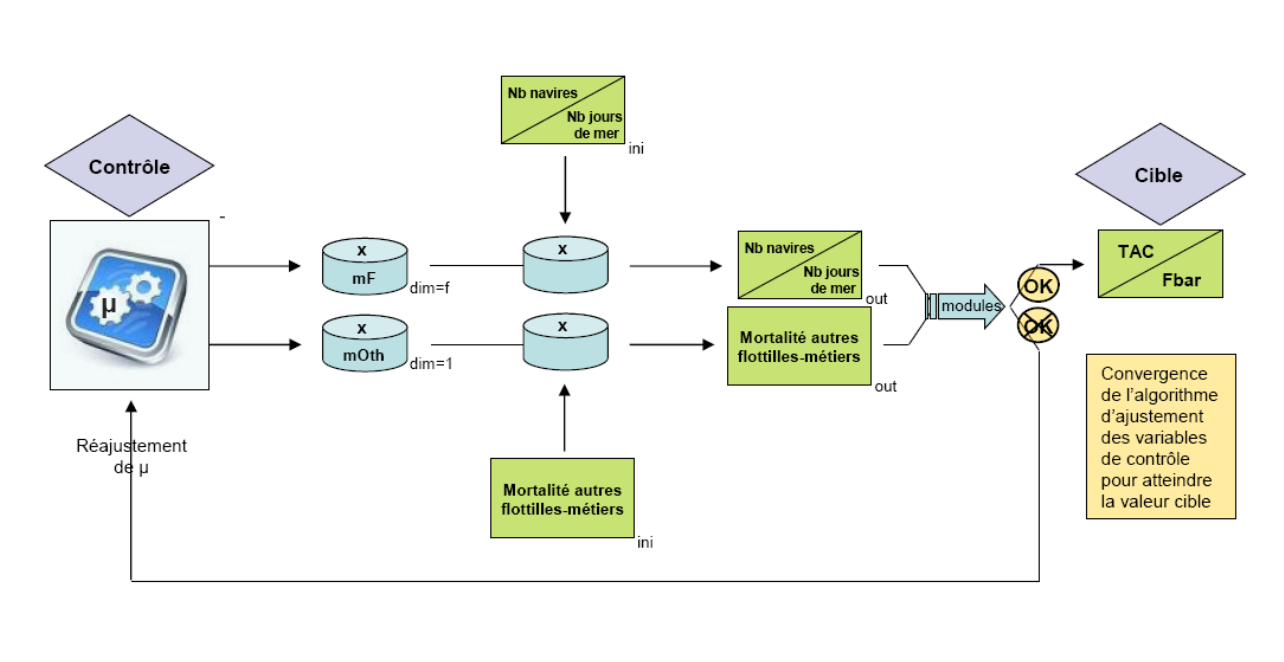
\includegraphics[width = 17cm]{figures/Gestion_module.png}
\end{center}
\caption{Fonctionnement du module "Gestion" pour les options d'atteinte de TAC et de Fbar}
\label{fig:gest_mod}
\end{figure}

Les perspectives quant à l'enrichissement du module par de nouvelles options de gestion (potentiellement apportées par l'intermédiaire d'un module complémentaire de simulation de comportement)  sont très nombreuses. Il est ainsi envisageable d'offrir la possibilité de définir des règles de variation des multiplicateurs (par exemple, en fonction de la rentabilité),  ou de multiplier les paramètres "cible" (ajout de la SSB,...), ou encore d'intégrer des contraintes sur les variations d'une année sur l'autre ou sur les valeurs limites des paramètres affectés (variation annuelle majorée de TAC, seuil minimal acceptable pour  l'EBE,...).

\subsection{Module "Réplicat"}

Le rôle de ce module est d'intégrer une variabilité dans les sorties du modèle en tirant parti des incertitudes considérées pour certaines variables (par le biais du module "Stochasticité", l'illustration évidente étant la donnée de recrutement). Comme son nom l'indique, il va procéder par réplication multiple des simulations afin d'obtenir pour chaque indicateur un jeu de valeurs permettant, par exemple, d'aboutir  à l'estimation d'une moyenne, d'une variance, ou bien encore d'un intervalle de confiance des projections.

Une schématisation de la façon dont le modèle  actuel fait collaborer les modules "Recrutement" et "Réplicat" (aussi appelé abusivement "Bootstrap") est représentée en figure \ref{fig:recru_mod}. On distingue d'abord parmi les paramètres d'entrée les variables qui évolueront entre deux répétitions (variables stochastiques) de celles qui resteront inchangées (variables non stochastiques). Comme on l'a vu précédemment, les variables stochastiques peuvent être de trois types : des variables issues d'un tirage aléatoire dans un historique (avec possibilité de pondérer les éléments le composant), des variables incarnant une réalisation d'une variable aléatoire donnée avec des paramètres donnés, et un cas particulier de variable (de recrutement) issue d'une relation Stock-Recrutement avec addition d'un bruit paramétré. Toutes ces variables prennent part à la simulation opérée par le modèle bio-économique, et si le module "Bootstrap" est activé, un certain nombre d'itérations (déterminé par l'utilisateur) est effectué, chaque sortie étant ainsi conservée en vue des traitements post visant à considérer (ou simplement à estimer) leur variabilité.  

\begin{figure}
\begin{center}
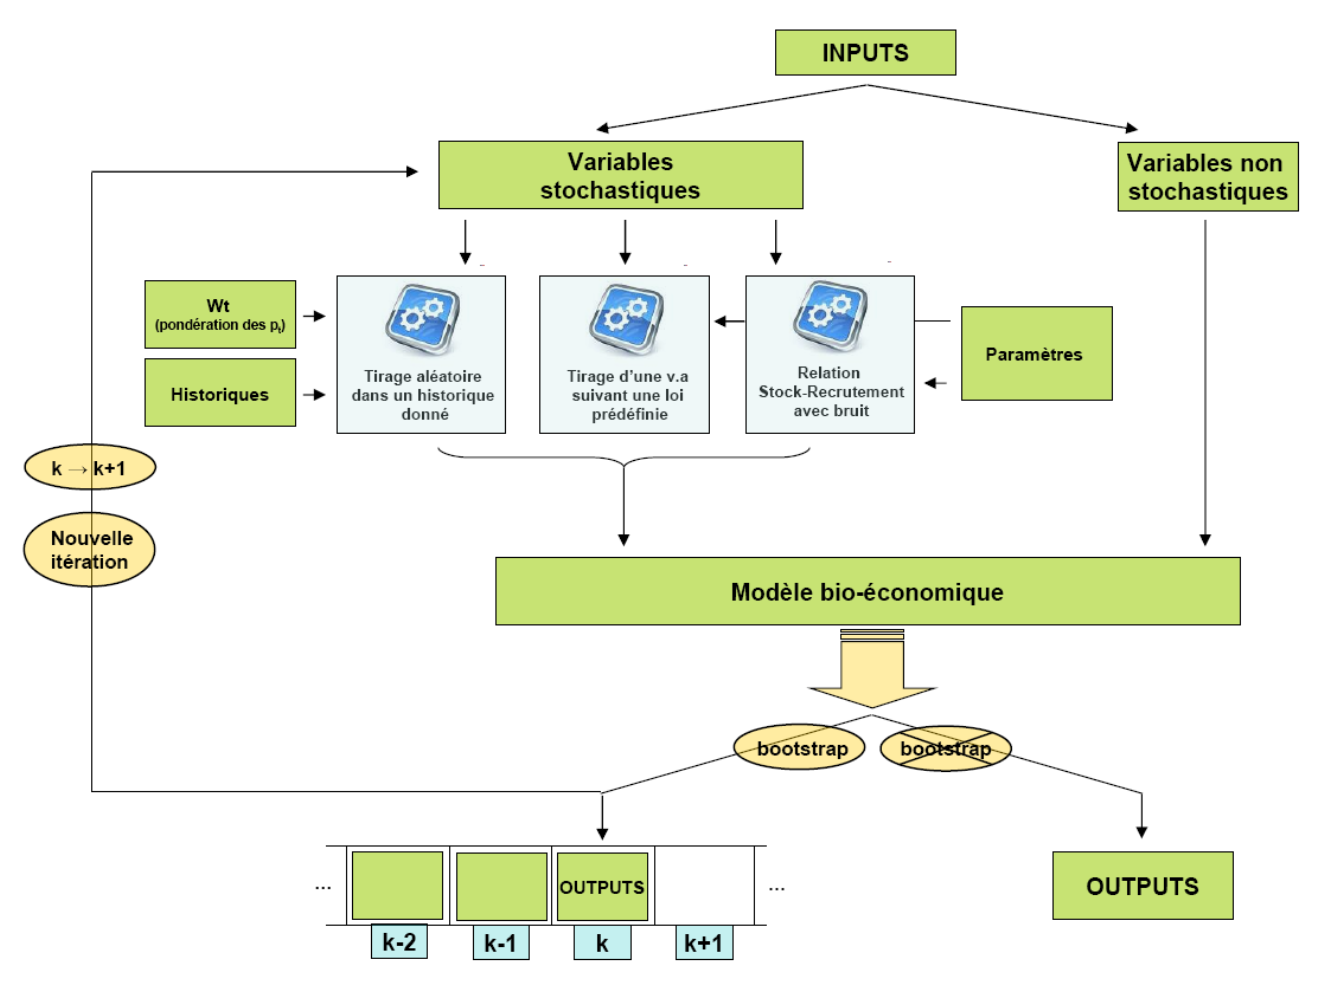
\includegraphics[width = 17cm]{figures/Recru_module.png}
\end{center}
\caption{Fonctionnement des modules "Recrutement" et "Bootstrap"}
\label{fig:recru_mod}
\end{figure}


\end{document}